%
% clam.tex -- master LaTeX file for 'CLAM: The Concise Linear Algebra Manipulation Language'
%
\newcommand{\sys}{CLAM}
\newcommand{\longtitle}{\sys{}: The Concise Linear Algebra Manipulation Language}
\newcommand{\authorlist}{Jeremy Andrus and Robert Martin and Kevin Sun and Yongxu Zhang}
\newcommand{\authoremails}{\{jca2119, rdm2128, kfs2110, yz2419\}@columbia.edu}

% Build Project proposal only (default for now)
\ifcsname ifproposal\endcsname\else
  \expandafter\let\csname ifproposal\expandafter\endcsname
                  \csname iftrue\endcsname
\fi
% Build Language Reference Manual only
\ifcsname ifrefman\endcsname\else
  \expandafter\let\csname ifrefman\expandafter\endcsname
                  \csname iffalse\endcsname
\fi
\ifcsname ifbook\endcsname\else
  \expandafter\let\csname ifbook\expandafter\endcsname
                  \csname iffalse\endcsname
\fi

% Document Class
\ifbook
  \documentclass[10pt,letterpaper,titlepage,onecolumn,oneside]{book}
\else
  \documentclass[10pt,letterpaper,onecolumn,oneside]{article}
\fi

\usepackage[margin=1.0in]{geometry}
\usepackage[utf8x]{inputenc}
\usepackage{ucs}
\usepackage{amsmath}
\usepackage{amsfonts}
\usepackage{amssymb}
\usepackage[usenames,dvipsnames]{color}
\usepackage{listings}
\usepackage[font=scriptsize,caption=false]{subfig}
\usepackage{underscore}
% hyphenat redefines "BreakableUnderscore", so I need
% to do some LaTeX gymnastics to make it work...
\makeatletter
\let\BreakableUnderscore\@undefined
\makeatother
\usepackage{hyphenat}
\usepackage{wrapfig}
\usepackage{lastpage}
\usepackage{balance}
\usepackage{cite}
\usepackage{pdfsync}
\usepackage[colorlinks=false,
    pdftitle={\longtitle{}},
    pdfborder={0 0 0},
    pdfauthor={\authorlist{}},
    pdfdisplaydoctitle=true,
    plainpages=false]{hyperref}
\usepackage{breakurl}
\usepackage{multirow}
\usepackage{pgfgantt}

\setlength{\parindent}{0in}
\addtolength{\parskip}{\baselineskip}

% other useful commands
\newcommand{\comment}[1]{}

\begin{document}

% this usually saves about a line-or-two by squeezing inter-sentence space
%\frenchspacing

\title{\longtitle{}}
\author{\authorlist{}\\\authoremails{}\\\\Columbia University\\COMS W4115: Programming Languages and Translators}
\maketitle

% Body of the paper in different files
\ifproposal
  % Project Proposal
  \section*{Language Proposal}

\definecolor{DarkBlue}{rgb}{0.0, 0.08, 0.65}
\definecolor{DarkRed}{rgb}{0.65, 0.08, 0.0}
\definecolor{DarkGreen}{rgb}{0.08, 0.35, 0.08}
\definecolor{Grey}{rgb}{0.55, 0.55, 0.55}
\definecolor{Yellow}{cmyk}{0.0, 0.08, 0.5, 0.3}
\definecolor{Brown}{rgb}{0.55, 0.27, 0.08}
\definecolor{LightBlue}{cmyk}{0.8, 0.1, 0.0, 0.1}
\lstdefinelanguage{PLTF11}{
    classoffset=0,
	morekeywords={somethingsomethingsomething},
    keywordstyle={\color{Yellow}\itshape\bfseries},
    classoffset=1,
    morekeywords={Uint8,Uint16,Uint32,Int8,Int16,Int32,Angle,Matrix,Image,Kernel},
    keywordstyle={\color{DarkBlue}\bfseries},
    classoffset=2,
	morekeywords={imgread,imgwrite},
	keywordstyle={\color{Brown}},
	otherkeywords={:=,**,=,|,:},
	moredelim=*[s][\color{LightBlue}]{\#[}{]},
	moredelim=*[s][\color{DarkGreen}\itshape]{\$(}{)},
    morecomment=[l]{//},
    commentstyle={\color{Grey}\bfseries},
    morestring=[b]",
    stringstyle={\color{DarkRed}},
    sensitive=true,
}

\sys{} is a linear algebra manipulation language specifically targeted for
image processing. It provides an efficient way to express complex image
manipulation algorithms through compact matrix operations. Traditional image
processing is performed using a language such as C, or C++. Algorithms in these
languages are quite complex and error-prone due to the large number of lines of
code required to implement something as conceptually simple as, "make this image
blurry." The complexity arises from the need to perform elaborate calculations
on every pixel in an image. For example, to blur an image you first need to
calculate the luminance of the pixel (from the red, green, and blue channels),
then you need to mathematically combine this with the luminance of adjacent pixels,
and finally re-calculate red, green, and blue values for an output image.

\sys{} will simplify image processing, and more generally linear algebra, through
domain-specific data types and operators. The basic data type in \sys{} is a 
\texttt{Matrix}. Matrices can be manipulated by operators that perform functions
such as matrix multiplication, or rotation. An \texttt{Image} is another \sys{}
data type which is expressed as a collection of matrices, or channels. For example,
when reading an image into memory, \sys{} creates a \emph{Red}, \emph{Green}, and
\emph{Blue} channel automatically. Additional Image channels can either be assigned,
or calculated using an expression syntax which defines a calculation involving the
values of other, previously defined, channels. The basic image processing operator
in \sys{} is the convolution operator. This operator takes a channel and a
\texttt{Kernel}, another basic data type, and outputs an \texttt{Image}. This
operator convolves each \texttt{Matrix} within the \texttt{Kernel} with the input channel,
and collects the resulting output channels into an \texttt{Image}.

Two primary use cases of \sys{} are basic image information extraction, and
filtering. The compact syntax and powerful basic data types of \sys{} will make
information extraction, such as finding all the edges in an image, simple, compact,
and easy to read.

\subsection*{Features}
\sys{} uses implicit loops, i.e. there is no explicit looping construct in the
language. Loops are implicitly defined by per-pixel matrix or convolution
operations. Additionally, \sys{} automatically determines or calculates image and matrix
dimensions. There is no need to explicitly size these data types. This further
reduces complexity, and eliminates frequent mistakes such as going beyond array
bounds in a calculation.

\subsection*{Example Syntax}

The goal of the \sys{} syntax will be to make conceptually simple image
manipulations into simple language constructs. For instance, convolutions make
frequent use of constant matrices, so our language will provide a simple way
to specify them, such as:
\begin{lstlisting}[language=PLTF11]
    Matrix sobelGy := { +1 +2 +1 |  0  0  0 | -1 -2 -1 };
\end{lstlisting}

Another common image processing technique is performing the same calculation
on every pixel in the image. An example of this is calculating the luminance
of a pixel from the red, green, and blue channels. \sys{} makes this calculation
simple and compact by defining an additional image channel. Assuming there exists
an instance of a \texttt{Image} variable named, \emph{myimg}, a channel can be
added to the image with:
\begin{lstlisting}[language=PLTF11]
    Int32 myimg:Luminance := #[ (3*Red + 6*Green + 1*Blue) / 10 ];
\end{lstlisting}
Where the expression within \texttt{\#[ \ldots ]} is evaluated once for every
pixel in the \texttt{Image}. The \emph{Red}, \emph{Green}, and \emph{Blue} variables
correspond to previously defined channels in \emph{myimg}, and their values during
expression evaluation will be the value of the corresponding channel at the current
pixel location.

Image processing also frequently involves describing a series of operations that
should be carried out for each pixel, and then repeating it for every pixel in an
image. \sys{} makes it simple to describe this process through the \texttt{Kernel}
data type and the convolution operator. Here is an example of how one might perform
a Sobel edge detector in the \sys{} language:
\lstinputlisting[language=PLTF11,numbers=left,frame=single]{src/sobel.imp}

\else
  
\definecolor{clamLightBlue}{cmyk}{0.8, 0.1, 0.0, 0.1}
\definecolor{clamDarkBlue}{rgb}{0.0, 0.08, 0.65}
\definecolor{clamDarkRed}{rgb}{0.65, 0.08, 0.0}
\definecolor{clamDarkGreen}{rgb}{0.08, 0.35, 0.08}
\definecolor{clamYellow}{cmyk}{0.0, 0.08, 0.5, 0.3}
\definecolor{clamPurple}{rgb}{0.58, 0.0, 0.83}
\definecolor{clamBrown}{rgb}{0.55, 0.27, 0.08}
\definecolor{clamGrey}{rgb}{0.55, 0.55, 0.55}
\lstdefinelanguage{CLAM}{
    classoffset=0,
    keywordstyle={\color{clamYellow}\bfseries}, % default style (used by 'otherkeywords')
    morekeywords={somethingsomethingsomething},
    classoffset=1,
    morekeywords={Uint8,Uint16,Uint32,Int8,Int16,Int32,Calc,Angle,Image,Kernel},
    keywordstyle={\color{clamDarkRed}\bfseries},
    classoffset=2,
    morekeywords={imgread,imgwrite},
    keywordstyle={\color{clamPurple}\bfseries},
    classoffset=3,
    otherkeywords={=,|,\,,:,:=,**,@},
    morecomment=[l]{//},
    morecomment=[n]{/*}{*/},
    commentstyle={\color{clamGrey}\bfseries},
    morestring=[b]",
    stringstyle={\color{clamBrown}},
    moredelim=*[s][\color{clamLightBlue}]{\#[}{]\#},
    moredelim=*[s][\color{clamBrown}]{[}{]},
    moredelim=*[s][\color{clamDarkGreen}]{\{}{\};},
    sensitive=true,
    showstringspaces=false,
    showspaces=false,
    showtabs=false,
    frame=single,
    numbers=left,
    basicstyle=\ttfamily,
}


  % Adapted from vim Ocaml syntax highlighting

\definecolor{ocamlLightBlue}{cmyk}{0.8, 0.1, 0.0, 0.1}
\definecolor{ocamlDarkBlue}{rgb}{0.0, 0.08, 0.65}
\definecolor{ocamlDarkRed}{rgb}{0.65, 0.08, 0.0}
\definecolor{ocamlDarkGreen}{rgb}{0.08, 0.35, 0.08}
\definecolor{ocamlYellow}{cmyk}{0.0, 0.08, 0.5, 0.3}
\definecolor{ocamlPurple}{rgb}{0.58, 0.0, 0.83}
\definecolor{ocamlBrown}{rgb}{0.55, 0.27, 0.08}
\definecolor{ocamlGrey}{rgb}{0.55, 0.55, 0.55}
\lstdefinelanguage{OCaml}{
    classoffset=0,
    keywordstyle={\color{ocamlPurple}\bfseries},
    morekeywords={somethingsomethingsomething},
    classoffset=1,
    morekeywords={and,as,assert,class,constraint,else,exception,external,fun,function,in,inherit,initializer,land,lazy,let,match,method,module,mutable,new,of,open,parser,private,raise,rec,then,try,type,val,virtual,when,while,with,do,value},
    keywordstyle={\color{ocamlDarkRed}\bfseries},
    classoffset=2,
    morekeywords={true,false,array,bool,char,exn,float,format,format64,int,int32,int64,lazy\_t,list,nativeint,option,string,uint},
    keywordstyle={\color{ocamlDarkBlue}\bfseries},
    classoffset=3,
    morekeywords={StringMap,String,List,Printf,Lexing,Scanner,Map,Make,Pervasives,Failure,VarMap,Parser,Ast},
    keywordstyle={\color{ocamlDarkGreen}},
    classoffset=4,
    otherkeywords={asr,lor,lsl,lsr,lxor,mod,not,::,;,|,@,->,<-,[],:=,;;,^,&&},
    morecomment=[l]{//},
    morecomment=[n]{(*}{*)},
    commentstyle={\color{ocamlGrey}\bfseries},
    morestring=[b]",
    stringstyle={\color{ocamlBrown}},
    moredelim=*[s][\color{ocamlBrown}]{'}{'},
    sensitive=true,
    showstringspaces=false,
    showspaces=false,
    showtabs=false,
    numbers=left,
    frame=single,
    breaklines=true,
    basicstyle=\ttfamily\scriptsize,
}


  \ifrefman
    % Language Reference Manual
    \section*{Language Reference Manual}
    \newcommand{\startsyn}{\begin{center}\begin{tabular}{l}}
\newcommand{\stopsyn}{\end{tabular}\end{center}}

\section{Introduction}
The \sys{} programming language is a linear algebra manipulation language
specifically targeted for image processing. It provides an efficient way to
express complex image manipulation algorithms through compact matrix
operations. \sys{} programs are first compiled into a ''C`` module which is
further compiled into a machine binary by an existing C compiler. This two-step
process is completely automated by the \sys{} compiler, and by default no C code
is output (this can be changed with compiler arguments - see section~\ref{sec:compiling}).

This language reference is inspired by the C reference manual~\cite{DBLP:KernighanR88}.
It details the syntax of the \sys{} language.

\section{Lexical Conventions}
\label{sec:lex}

\subsection{Tokens}
\label{ssec:tokens}
The tokens in \sys{} are broken down as follows: reserved
keywords, identifiers, constants, control characters, and operators.
The end of a token is defined by the presence of a newline, space,
tab character (whitespace), or other character that
cannot possibly be part of the current token.

\subsection{Comments}
\label{ssec:comments}
Comments are demarcated with an opening /* and closing */, as in C.
Any characters inside the comment boundaries are ignored. Comments
can be nested.

\clearpage % FORMAT HACK!
\subsection{Keywords}
\label{ssec:keywords}
The reserved keywords in \sys{} are:
\begin{center}\begin{tabular}{l l l l}
Image & imgread & Int8 & Uint8\\
Kernel & imgwrite & Int16 & Uint16\\
Calc & Angle & Int32 & Uint32
\end{tabular}\end{center}

\subsection{Identifiers}
\label{ssec:identifiers}
Identifiers are composed of an upper or lower-case letter immediately
followed by any number of additional letters and/or digits. Identifiers
are case sensitive, so ``foo'' and ``Foo'' are different identifiers.
Identifiers cannot be keywords, and cannot start with a digit.

\subsection{Constants}
\label{ssec:constants}
In \sys{} there are 3 types of constants: numeric constants,
calculation constants, and string literals.

\subsubsection{Numeric Constants}
\label{sssec:numericconstants}

\emph{Integers} are repesented by a series of number characters.
% the negative sign is dealt with by the unary '-' operator

Angles are represented by a series of number characters with an
optional period character.

\subsubsection{Calculation Constants}
\label{sssec:calcconstants}
Matrix calculation constants are represented by an opening curly brace, followed
by a series of \emph{numeric-expressions} separated by whitespace or
comma characters. The comma  characters represents the division between
the rows of the matrix. Each row must have the same number of
\emph{numeric-expressions}, but the matrix need not be square.

A calculation constant may also have an optional fraction preceding it,
which indicates that every value in the matrix should be multiplied
by that fraction. The fraction will be expressed as an opening
bracket character, a \emph{numeric-expression} representing the
numerator, a forward-slash character, a \emph{numeric-expression}
representing the denominator, and a closing bracket character.

\startsyn
\texttt{\{} \emph{numeric-expr} \emph{numeric-expr} \ldots \texttt{,} \emph{numeric-expr} \emph{numeric-expr}\ldots \texttt{\}} \\
\texttt{[}\emph{numeric-expr} \texttt{/} \emph{numeric-expr} \texttt{]}\texttt{\{} \emph{numeric-expr} \emph{numeric-expr} \ldots \texttt{,} \emph{numeric-expr} \emph{numeric-expr}\ldots \texttt{\}}
\stopsyn

The following is an example of a calculation constant.
\begin{lstlisting}[language=CLAM,escapechar=\%]
Calc sobelGy := [1 / 9]{1 3 1 , 2 -5 2 , 1 3 1 };
\end{lstlisting}

\subsubsection{String Literals}
\label{sssec:strings}

String constants are demarcated by double quote characters or single
quote characters. Consecutive string constants will be automatically
appended together into a single string constant.
String constants may contain escaped characters. Escaped characters begin with
a backslash, \texttt{\textbackslash}, and are followed by either an octal,
hexadecimal or base-10 integer value. The following escaped characters are also supported:
\startsyn
\texttt{\textbackslash{}n} (newline)\\
\texttt{\textbackslash{}t} (tab)\\
\texttt{\textbackslash{}b} (break)\\
\texttt{\textbackslash{}r} (carriage-return)\\
\stopsyn

\startsyn
\texttt{"}\emph{string-constant}\texttt{"} \\
\texttt{"}\emph{string-constant}\texttt{"} \texttt{"}\emph{string-constant}\texttt{"} \ldots \\
\stopsyn

\section{Meaning of Identifiers}
\label{sec:identmeaning}

\subsection{Basic Types}
\label{ssec:types}
There are three basic types defined by the \sys{} language.
Type identifiers always begin with an upper-case letter followed by a sequence
of zero or more legal identifier characters. The list of built-in types is as follows:
\startsyn
\texttt{Image} \\
\texttt{Calc} \\
\texttt{Kernel}
\stopsyn 

\subsubsection{Atom Types}
\label{sssec:atomtypes}
The \texttt{Calc} type may be further modified
to specify individual element, or ``atom'' types. This specifies the type
of the resulting calculation performed by a \texttt{Calc} object (either CString or Matrix --
see section~\ref{ssec:calc}). When calculation results exceed the bounds of the specified type,
values are clamped (set to the max or min value appropriately).
An \emph{atom-type} identifier is denoted using the \texttt{<} and \texttt{>}
characters immediately following the identifier of the object whose atom type
is being specified:
\startsyn
\texttt{Calc} \emph{identifier}\texttt{<}\emph{atom-type}\texttt{>}
\stopsyn
Legal \emph{atom-type}s are as follows:
\startsyn
Uint8 \\
Uint16 \\
Uint32 \\
Int8 \\
Int16 \\
Int32 \\
Angle
\stopsyn
In the absence of an atom-type specification, the atom-type defaults to Uint8,
which implies a range of integers from 0-255 inclusive. (This is also the atomic-type
for the default \emph{Red}, \emph{Green} and \emph{Blue} channels.)


\section{Objects and Definitions}
\label{sec:objdef}
An \emph{object} in \sys{} is either a named collection of Channels, called an
\texttt{Image}, or a named collection of calculation bases, called a
\texttt{Kernel}. A Channel is a mathematical matrix of numeric values
whose individual components are not directly accessible via \sys{} language
semantics -- Channel values are manipulated via the convolution
operator (see~\ref{ssec:convolutionop}). A calculation basis, known as a
\texttt{Calc}, is either a calculation constant
(see~\ref{sssec:calcconstants}) or a calculation expression (see~\ref{ssec:escapedC}).

\subsection{\texttt{Calc} objects}
\label{ssec:calc}
A  \texttt{Calc} object is an immutable object initialized with the \texttt{:=} assignment operator
(see section~\ref{sssec:colonequalop}). Its assigned value is either a CString (section~\ref{ssec:escapedC}),
or a calculation constant (\emph{matrix} - section~\ref{sssec:calcconstants}). The calculation
described by a \texttt{Calc} object will be performed for each pixel in an \texttt{Image} Channel.
The calculation is performed using either the convolution operator (section~\ref{sssec:convolutionop}),
or the channel composition operator (section~\ref{sssec:barequalop}).

\subsection{\texttt{Image} objects}
\label{ssec:images}
An \texttt{Image} is a collection of named Channels. Channels can
be dynamically added \comment{or removed} using the channel composition
operator (see section~\ref{sssec:barequalop}, or by assigning to a previously
undeclared Channel name. 

For example, to create a gray-scale image from a single, pre-existing
Channel:
\begin{lstlisting}[language=CLAM,escapechar=\%]
Image outImg;
outImg:Red = calcImg:G;
outImg:Green = calcImg:G;
outImg:Blue = calcImg:G;
\end{lstlisting}

\subsection{\texttt{Kernel} objects}
\label{ssec:kernels}
A \texttt{Kernel} is an ordered collection of calculation bases which is used by the convolution
operator (see section~\ref{ssec:convolutionop}). Each calculation must to be identified with a \texttt{Calc}
identifier, but the underlying basis can be either
a matrix calculation constant (see~\ref{sssec:calcconstants}) or an escaped C expression
(see~\ref{ssec:escapedC}). A \texttt{Kernel} is composed either using the composition
operator (see section~\ref{sssec:barop}), or the \texttt{|=} assignment operator (see section~\ref{sssec:barequalop}).

To see how a \texttt{Kernel} is used in calculation, see section~\ref{ssec:convolutionop}.

\section{Expressions}
\label{sec:expressions}

\subsection{Primary Expressions}
\label{ssec:primaryexpresions}
\sys{} primary expressions can be identifiers, constants, or strings.
The type of the expression depends on the identifier, constant or string.

\subsection{Unary Operators}
\label{ssec:unaryoperators}
There are two unary operators in \sys{}, and they are only used with a
numeric-valued operand such as a numeric constant
(see~\ref{sssec:numericconstants}).
These expressions are grouped right-to-left:
\startsyn
\texttt{+}\emph{unsigned-integer} \\
\texttt{-}\emph{unsigned-integer}
\stopsyn

\subsubsection{\texttt{+} operator}
This operator forces the value of its numeric operand to be positive.
The resulting expression is of numeric type with a value equal to the
value of the numeric operand.

\subsubsection{\texttt{-} operator}
This operator forces the value of its numeric operand to be negative.
The resulting expression is of numeric type with a value equal to the
negative of the numeric operand.

\subsection{Channel/Calc Expresions}
\label{ssec:channelexpressions}
Channel and \texttt{Calc} types are the basis of \texttt{Image} and
\texttt{Kernel} objects respectively. There are several operators that
manipulate Channels and \texttt{Calc}s.

\subsubsection{\texttt{:} operator}
\label{sssec:colonop}
Extract, reference or assign an individual Channel in an image.
\startsyn
\emph{image-identifier}\texttt{:}\emph{channel-identifier}
\stopsyn
The resulting expression has a type corresponding to the
extracted Channel.

\subsection{Composition Operators}
\label{ssec:compositionops}
These operators compose an \texttt{Image} or \texttt{Kernel} from one
or more \texttt{Calc} objects.
All channel composition operators are left-to-right associative.

\subsubsection{\texttt{|} operator}
\label{sssec:barop}
Define of list of (one or more) \texttt{Calc}s. The resulting expression is a
\emph{multi-calc} expression, and can be assigned
to a \texttt{Kernel} object.
\startsyn
\texttt{|} \emph{calc-expression} \\
\emph{multi-calc-expression} \texttt{|} \emph{calc-expression} \\
\stopsyn
Note that \texttt{Calc}s are appended in order, and
subsequent operations may rely on this order.
Also note that even single \texttt{Calc} identifiers must be preceded by \texttt{|}

\subsection{\texttt{**} operator}
\label{ssec:convolutionop}

The convlution operator, or \texttt{**}, performs the calculations of a
\texttt{Kernel} on a Channel, and evaluates to a new \texttt{Image}. The
resulting \texttt{Image} will have a Channel for the result of each
(non-transient) calculation.
When a \texttt{Kernel} is evaluated, as many operations as possible are
parallelized to improve performance.

Parallelized calculations may depend on each other as long as the
dependent calculation is listed after its dependency when the \texttt{Kernel} is
defined, and the dependent calculation does not depend on more than
the current pixel of the required calculation.

Any channels marked with an \texttt{@} symbol are transient and
are not added to the result \texttt{Image}.

\subsection{Escaped ``C'' Expression}
\label{ssec:escapedC}

Escaped ``C'' expressions, or \emph{CStrings}, are snippits of ``C'' code
which will be run once for every pixel in an \texttt{Image} Channel. The
string may reference other Channels in the \texttt{Image} provided the
Channels have been previously defined. To reference a Channel within a
CString, the name of the Channel is used just like a local variable in C.
CStrings are used on the right side
of the \texttt{:=} operator when defining a Channel.

The escaped code must be a single expression
in C that will evaluate to the type defined by the containing \texttt{Calc} object.
The expression cannot contain the following characters/tokens:
\texttt{; \# \{ \} " ' /* */}. Parentheses may be used to group expressions or
cast objects, but all parenthesis within the expression must be matched.

\texttt{Calc} types and their C-equivalent types:
\begin{center}\begin{tabular}{l | l}
\sys type & equivalent C type \\
\hline
Uint8  & uint8_t \\
Uint16 & uint16_t \\
Uint32 & uint32_t \\
Int8  & int8_t \\
Int16 & int16_t \\
Int32 & int32_t \\
Angle  & float
\end{tabular}\end{center}

When the channel described by a CString must be evaluated,
every pixel value in the channel is calculated by evaluating the C expression.
When the expression is evaluated, every identifier corresponding to
another channel in the image will be replaced by the value of the
pixel in the same location in the referenced channel. Thus, if the C expression
contains the identifier \texttt{Red}, then when the channel is calculated
it will replace \texttt{Red} in the expression with the appropriate value
from the \texttt{Red} channel.

All standard C operators are available for use, as well as any library functions
defined in \texttt{math.h}. Although bracket characters are not allowed within
CStrings, the \emph{ternary} conditional operator, \texttt{a ? b : c} is allowed.
This enables more complex pixel value calculations such as thresholding and hysteresis.

\subsection{I/O Expressions}

\subsubsection{\texttt{imgread} expression}
\label{sssec:imgread}
The \texttt{imgread} expression reads in an \texttt{Image} object from
a known image format located on the file system. The expression results
in an \texttt{Image} object which can be assigned using the \texttt{=}
operator (see section~\ref{sssec:equalop}). The resulting \texttt{Image}
object has 3 Channels named \emph{Red}, \emph{Green}, and
\emph{Blue}. Each of the channels correspond to the red, green, and blue
image data read into the \texttt{Image} object. This expression is invoked
as a ``C'' style function, and expects 1 parameter: either the path of the
image file to read (expressed as a string constant); or the number of the
command-line argument, an integer 1 or greater.
\startsyn
\texttt{imgread(} \emph{string-constant} \texttt{|} \emph{integer} \texttt{)}
\stopsyn

\subsubsection{\texttt{imgwrite} expression}
\label{sssec:imgwrite}
The \texttt{imgwrite} expression writes out an \texttt{Image} object to a known
image format. It requires that the \texttt{Image} object has at least 3 named
\texttt{Channels}: \emph{Red}, \emph{Green}, and \emph{Blue}.
This expression has no type (null type), and is invoked as a ``C'' style function.
It expects 3 parameters: the first parameter is an \texttt{Image} identifier, the
second is the image format, and the third is the path to which the image
should be written (or an integer which represents a command-line argument, as for
\texttt{imgread}).
\startsyn
\texttt{imgwrite(} \emph{image-identifier} \texttt{,} \emph{string-constant} \texttt{,} \emph{string-constant} \texttt{|} \emph{integer} \texttt{)}
\stopsyn

\subsection{Assignment Expressions}
\label{ssec:assignment}

\subsubsection{\texttt{=} assignment operator}
\label{sssec:equalop}
Assigns the value of the right operand to the left operand, copying data as necessary.
The types of both operands must match. Cannot be used with \texttt{Calc}s, which are
defined once only (see \texttt{:=} below).

The type of this expression is equal to the type of the left operand, and assignment
operations may be chained together. For example:
\begin{lstlisting}[language=CLAM]
Image a;
Image b;
imgwrite(a = b = imgread("foo.jpg"), "png", "foo.png");
\end{lstlisting}

\subsubsection{\texttt{:=} assignment operator}
\label{sssec:colonequalop}
Assigns a calculation constant (see section~\ref{sssec:calcconstants}), or
escaped ``C'' expression (see section~\ref{ssec:escapedC}) to a \texttt{Calc}
object. Only used once for each \texttt{Calc}, with declaration.

\subsubsection{\texttt{|=} assignment operator}
\label{sssec:barequalop}
Add a single Channel or a (possibly one-member) list of \texttt{Calc}s object to an \texttt{Image} or
\texttt{Kernel} object. Assignments using this operator are ordered by statement
order, and subsequent operations can rely on this order.

\section{Statements}
\label{sec:statements}

Statements in \sys{} always end in a semi-colon. No statement
can return a value. All statements should either declare a variable,
define or modify the definition of a variable, execute
some calculation based on previously declared variables with
the result stored in previously declared variables, or write an image to a file.
"Statements" consisting of a lone r-value (an identifier,
channel reference, escaped-C string, matrix, or \texttt{imgread()} call)
will be accepted but will perform no useful action - they are evaluated but
their return values are discarded. Additionally, the \sys{} compiler may
optionally remove these statements as an optimization.

\section{Program Definition}
A program in the \sys{} language is simply a sequence of statements which
are executed in order.

\section{Scope Rules}
All identifiers in the \sys{} language are global.

In a CString that defines a channel, the existing channels
for an image will be in scope when the block is executed. Because
this block will be executed on every pixel, the name of the channel
will bind to the current pixel value for that channel. These bindings
will be resolved when the channel is calculated, not when it is
defined, and will be removed after calculation.

\section{Declarations}
All variables must be declared before they can be used. However,
variable declarations can be made at any point in a program.
A variable becomes usable after the end of the semi-colon of the statement
in which it is contained.

\section{Grammar}

\subsection{Expressions}

\begin{center}\begin{tabular}{l l}
\emph{expression}: & \emph{identifier}\\
& \emph{integer}\\
& \emph{literal-string}\\
& \emph{c-string}\\
& \emph{matrix}\\
& \emph{matrix-scale matrix}\\
& \emph{kernel-calc-list}\\
& \emph{channel-ref}\\
& \emph{identifier} \texttt{=} \emph{expression}\\
& \emph{channel-ref} \texttt{=} \emph{expression}\\
& \emph{channel-ref} \texttt{**} \emph{identifier}\\
& \emph{identifier} \texttt{|=} \emph{expression}\\
& \emph{library-function} \texttt{(} \emph{argument-list} \texttt{)}\\
\\
\emph{matrix-scale}: & \texttt{[} \emph{integer} \texttt{/} \emph{integer} \texttt{]}\\
\\
\emph{matrix}: & \texttt{\{} \emph{row-list} \texttt{\}}\\
& \emph{matrix-scale} \texttt{\{} \emph{row-list} \texttt{\}}\\
\\
\emph{row-list}: & \emph{matrix-row}\\
& \emph{row-list} \texttt{,} \emph{matrix-row}\\
\\
\emph{matrix-row}: & \emph{integer}\\
& \emph{matrix-row} \emph{integer}\\
\\
\emph{kernel-calc-list}: & \texttt{@}\emph{identifier}\\
& \texttt{|} \emph{identifier}\\
& \texttt{| @}\emph{identifier}\\
& \emph{kernel-calc-list} \texttt{|} \emph{identifier}\\
& \emph{kernel-calc-list} \texttt{| @}\emph{identifier}\\
\\
\emph{channel-ref}: & \emph{identifier}\texttt{:}\emph{identifier}\\
\\
\emph{argument-list}: & \emph{literal-string}\\
& \emph{argument-list} \texttt{,} \emph{literal-string}\\
\\
\emph{library-function}: & \texttt{imgread}\\
& \texttt{imgwrite}\\
\end{tabular}\end{center}

\subsection{Declarations}

\begin{center}\begin{tabular}{l l}
\emph{declaration}: & \texttt{Image} \emph{identifier}\\
& \texttt{Kernel} \emph{identifier}\\
& \texttt{Calc} \emph{identifier}\\
& \texttt{Calc} \emph{identifier}\texttt{<}\emph{atomic-type}\texttt{>}\\
\\
\emph{atomic-type}: & \texttt{Uint8}\\
& \texttt{Uint16}\\
& \texttt{Uint32}\\
& \texttt{Int8}\\
& \texttt{Int16}\\
& \texttt{Int32}\\
& \texttt{Angle}\\
\end{tabular}\end{center}


\subsection{Statements and Programs}

\begin{center}\begin{tabular}{l l}
\emph{statement}: & \emph{expression} \texttt{;}\\
& \emph{declaration} \texttt{;}\\
& \emph{declaration} \texttt{=} \emph{expression} \texttt{;}\\
& \emph{declaration} \texttt{:=} \emph{expression} \texttt{;}\\
\\
\emph{program}: & \emph{statement}\\
& \emph{statement} \emph{program}\\
\end{tabular}\end{center}




\clearpage
\section{Examples}

\subsection{Gaussian Blur}
Figure~\ref{fig:clamblur} shows an example \sys{} program which performs a Gaussian
blur on an input image. The input and resulting output images are shown in
Figures~\ref{fig:clamblurin} and~\ref{fig:clamblurout}.

\begin{figure}[hb!]
  \begin{center}
  \lstinputlisting[language=CLAM]{src/blur.clam}
  \caption{Gaussian Blur Implemented in \sys{}}
  \label{fig:clamblur}
  \end{center}
\end{figure}
{
  \captionsetup{justification=centering}
  \begin{figure*}[h!]
    \centering
    \subfloat[Input Image]{
      \includegraphics*[width=7.5cm]{figures/lena.png}\label{fig:clamblurin}
    }\hfill
    \subfloat[Blurred Output Image]{
      \includegraphics*[width=7.5cm]{figures/lena-blur.png}\label{fig:clamblurout}
    }\hfill
    \captionsetup{font=bf}
    \caption{Gaussian Blur \sys{} Example}
  \end{figure*}
}

\clearpage
\subsection{Image Segmentation}
Figure~\ref{fig:clamseg} shows an example \sys{} program which performs
basic image segmentation. Pixels with a luminance value greater than 200 are
displayed as red, pixels with a luminance less than or equal to 80 are displayed as blue,
and pixels in between are displayed as Green. The input and resulting output images are shown in
Figures~\ref{fig:clamsegin} and~\ref{fig:clamsegout}.

\begin{figure}[hb!]
  \begin{center}
  \lstinputlisting[language=CLAM]{src/segment.clam}
  \caption{Simple Image Segmentation Implemented in \sys{}}
  \label{fig:clamseg}
  \end{center}
\end{figure}
{
  \captionsetup{justification=centering}
  \begin{figure*}[h!]
    \centering
    \subfloat[Input Image]{
      \includegraphics*[width=7.5cm]{figures/lena.png}\label{fig:clamsegin}
    }\hfill
    \subfloat[Segmented Output Image]{
      \includegraphics*[width=7.5cm]{figures/lena-seg.png}\label{fig:clamsegout}
    }\hfill
    \captionsetup{font=bf}
    \caption{Image Segmentation \sys{} Example}
  \end{figure*}
}

    \clearpage
  \else
    % Final Project report is the default output here
    \tableofcontents
    \chapter{Introduction}
\label{chap:intro}

\sys{} is a linear algebra manipulation language specifically targeted for
image processing. It provides an efficient way to express complex image
manipulation algorithms through compact matrix operations. Traditional image
processing is performed using a language such as C, or C++. Algorithms in these
languages are quite complex and error-prone due to the large number of lines of
code required to implement something as conceptually simple as, "make this image
blurry." The complexity arises from the need to perform elaborate calculations
on every pixel in an image. For example, to blur an image you first need to
calculate the luminance of the pixel (from the red, green, and blue channels),
then you need to mathematically combine this with the luminance of adjacent pixels,
and finally re-calculate red, green, and blue values for an output image.

\sys{} simplifies image processing, and more generally linear algebra, through
domain-specific data types and operators. A basic data type in \sys{} is a
\texttt{Calc}, which can either be a \emph{Matrix} or a \emph{CString}.
Matrices can be variable sized with an optional rational coefficient, and are
used in image convolution operations. CStrings are simple calculations
based on previously defined channels and basic C math operations such as \texttt{sqrt}
or \texttt{atan}.

An \texttt{Image} is another \sys{} data type which is expressed as a collection
of channels. For example, when reading an image into memory, \sys{} creates a
\emph{Red}, \emph{Green}, and \emph{Blue} channel automatically. Additional
Image channels can be assigned from other images, or calculated
using an expression syntax that defines a calculation involving the
values of other, previously defined, channels. The basic image processing operator
in \sys{} is the convolution operator. This operator takes an \texttt{Image} channel and a
\texttt{Kernel}, an ordered collection of \texttt{Calc} objects. This
operator convolves each \texttt{Matrix} within the \texttt{Kernel} with the input channel,
and runs each CString calculation on the input channel in the order they were defined in
the \texttt{Kernel}. It then collects the resulting output channels into a new \texttt{Image}.

Two primary use cases of \sys{} are basic image information extraction, and
filtering. The compact syntax and powerful basic data types of \sys{} make
information extraction, such as finding all the edges in an image, simple, compact,
and easy to read.


    \chapter{Language Tutorial}
\label{chap:tutorial}

\section{Input and Output}

\sys{}'s basic I/O operators are \texttt{imgread} and \texttt{imgwrite}, and every program
will have to call them at least once each to do anything useful. \texttt{imgread}
takes a filename (or integer, see below) as its sole argument and returns an \texttt{Image}.
\texttt{imgwrite} take an \texttt{Image}, a format, and filename (or integer).

\subsection{Your first program}

Using only I/O operators, you can already write a simple program that copies an image from
one location to another. Or, if the output is in a different format than the input,
you have a simple image converter. In either case, you only need two lines of code!

\begin{lstlisting}[language=CLAM,escapechar=\%]
Image input = imgread("source.jpg");
imgwrite(input, "png", "dest.png");
\end{lstlisting}
\ldots or 1 if you're tricky
\begin{lstlisting}[language=CLAM,escapechar=\%]
imgwrite(imgread("source.jpg"), "png", "dest.png");
\end{lstlisting}

\subsection{Using command-line arguments}

This program only copies from \texttt{"source.jpg"} to \texttt{"dest.png"} which is not
very useful.
You'd need to edit the code and recompile to change the source and destination.
To avoid this problem, \texttt{imgread} and \texttt{imgwrite} can both be called with integers
which refer to items in the command-line argument list, giving your code much greater
flexibility. (\sys{} will automatically enforce the correct number of command-line arguments.)

\begin{lstlisting}[language=CLAM,escapechar=\%]
imgread(1); /* Get filename from argv[1]*/
imgwrite(input, "png", 2); /* Get filename from argv[2]*/
\end{lstlisting}

\section{Compiling and Running Your Program}
\label{sec:compiling}

In order to generate binaries from your \sys{} program, you will need the \texttt{g++} compiler
installed and available in your default \texttt{PATH}. This is because \sys{} uses C/C++ as its
compile target, and leverages existing C/C++ compilers to generate and optimize machine-dependent code.
You can compile your clam program by simply passing your file to \texttt{clam} as the sole argument.
This will automatically output a binary to \texttt{a.out}. You can also specify the name of
the binary with the \texttt{-o} flag, and pass in the source file path with \texttt{-i}.
For example:
\begin{itemize}
  \item \texttt{./clam prog1.clam}
  \item \texttt{./a.out source.jpg dest.png}
  \item \texttt{./clam -i prog1.clam -o copyimg}
  \item \texttt{./copyimg source.jpg dest.png}
\end{itemize}

The full set of options to the \sys{} compiler can be found using the \emph{--help} option, and is
reproduced below:
\begin{lstlisting}[language=make,basicstyle=\ttfamily]
CLAM v0.1
Usage: clam {options} [{<} inputfile]
Options are:
  -o <filename> Specify the output file
  -i <filename> Specify the input file
  -c            Output generated C only
  -t            Print AST debugging information
  -help         Display this list of options
  --help        Display this list of options
\end{lstlisting}

\section{Basic Types}

\subsection{Channels}

\emph{Channels} are arrays of values associated each pixel in an \texttt{Image}.
For example, each pixel in an \texttt{Image} usually has \emph{Red}, \emph{Green}, and \emph{Blue} values
associated with it, and we can further define \emph{Luminosity}, \emph{Hue}, \emph{Saturation} etc.
Thus we can refer to the \emph{Red} channel or the \emph{Saturation} channel of an \texttt{Image}.

When first read into \sys{}, \texttt{Image}s come with three default Channels:
\texttt{Red}, \texttt{Green}, and \texttt{Blue}. These can be accessed using the \texttt{:} (colon) operator.
The values in one Channel can be copied to another using the \texttt{=} (equals) operator.
If the Channel on the left-hand side is undefined, it is created dynamically.

The following program uses a \texttt{temp} channel to swap the \texttt{Red} and \texttt{Blue} values of an image:

\begin{lstlisting}[language=CLAM,escapechar=\%]
Image img1 = imgread(1);

img1:temp = img1:Blue;
img1:Blue = img1:Red;
img1:Red = img1:temp; /* swap channels */

/*Only Red, Green, and Blue channels are written:*/
imgwrite(img1, "jpg" ,2);
\end{lstlisting}

\subsection{Calculations}

While the equals operator is enough to create new channels that are copies of old ones,
\texttt{Calc} objects allow you to create new Channels via calculation.
The \texttt{:=} (colon-equals) operator is used to define \texttt{Calc}s object.
Once defined, a \texttt{Calc} object cannot be redefined.
A \texttt{Calc} can be assigned an \emph{atomic type} such as \texttt{<Uint16>} or \texttt{<Angle>},
and all values resulting from that calculation will be clamped to the appropriate range.
The default type is \texttt{<Uint8>}, which corresponds to a range of 0-255.
  
\texttt{Calc} objects can be defined in two ways - as \emph{escaped-C strings} (\emph{CStrings}) or as \emph{matrices}.

CString \texttt{Calc}s are enclosed in \texttt{\#[\ldots]\#} brackets. These strings can contain basic mathematical
operators and functions, as well as references to other Channels. A \texttt{Calc}
defined in this manner can be applied to an \texttt{Image} using the \texttt{|=} (or-equal) operator,
provided that the \texttt{Image} has all the requisite Channels,
thereby creating a new Channel with the same name as the \texttt{Calc}. The values of this new
Channel will be calculated according
to the contents of the string. (It follows that anonymous \texttt{Calc}s are not allowed.)\\

\begin{lstlisting}[language=CLAM,escapechar=\%]
/* Define a calculation for Luminosity */
Calc Lum<Uint8> := #[(3*Red + 6*Green + 1*Blue) / 10]#;
Calc Zero := #[0]#;

Image srcimg = imgread(1);
/* Add luminosity channel to the Image */
srcimg |= Lum;

/* Add a 'black' channel to the Image, named 'Zero' */
srcimg |= Zero;

/* The following is invalid - no name! */
srcimg |= #[Red + Green + Blue]#;

/* Calcs cannot be redefined! */
Lum := #[Red * Green * Blue]#
\end{lstlisting}

\emph{Matrix} \texttt{Calc}s can be of any size, and are represented as lists of numbers enclosed in
\texttt{\{\ldots\}} braces. Rows are separated by commas, and the \emph{Matrix} is optionally preceded by
a scaling factor of the form \texttt{[} \emph{numerator} \texttt{/} \emph{denominator} \texttt{]}.
Matrices represent a weighted (and scaled) sum of values in the neighborhood of a pixel.
Because matrix \texttt{Calc}s cannot be calculated with a simple ``for loop,'' over all pixels,
they cannot be applied
directly to \texttt{Image}s. However they can be added to \texttt{Kernels} and then \emph{convolved}
with \texttt{Image}s (see section~\ref{sec:tutorial:kernels}) and are useful in a wide range of applications.\\

\begin{lstlisting}[language=CLAM,escapechar=\%]
Calc Avg<Uint8> := [1/9] { 1 1 1, 1 1 1, 1 1 1 };
/* This matrix averages the values in a 3x3 square
	centered on a given pixel */

/* This doesn't work: */
srcimg |= Avg;
\end{lstlisting}

\subsection{Kernels}\label{sec:tutorial:kernels}

\texttt{Kernel} are ordered collections of \texttt{Calc}s. They are defined with the \texttt{=} (equals) operator
and a list of \texttt{Calc}s separated by the | (or) operator. More \texttt{Calc}s can be added to
a \texttt{Kernel} afterwards using the \texttt{|=} (or-equal) operator. A \texttt{Calc} in a \texttt{Kernel}
can be prefixed with the \texttt{@} (at) symbol to indicate that it is an intermediate calculation
(see section~\ref{sec:tutorial:convolutions}).

\begin{lstlisting}[language=CLAM,escapechar=\%]
Calc sobelGx<Uint8> := {-1 0 +1, -2 0 +2, -1 0 +1};
Calc sobelGy<Uint8> := {+1 +2 +1, 0 0 0, -1 -2 -1};
Calc sobelG<Uint8> :=
    #[sqrt(sobelGx * sobelGx + sobelGy * sobelGy)]#;
Kernel k = | @sobelGx | @sobelGy | sobelG;
/* Calcs can refer to preceding Calcs in same kernel */

Calc sobelTheta := #[atan((float)sobelGx/(float)sobelGy)]#;
k |= sobelTheta; 
/* don't have to add all Calcs at once */
\end{lstlisting}

\section{Convolutions}\label{sec:tutorial:convolutions}

The \texttt{**} operator takes a Channel reference and a \texttt{Kernel}, and
applies the \texttt{Kernel}'s \texttt{Calc}s in sequence to the Channel.
Matrices are applied to the directly to the \texttt{Image} Channel specified,
while CStrings generally calculate a value using other Channels. Any Channel which has
already been calculated in the convolution may be used by a CString \texttt{Calc}.
The result of a convolution is an \texttt{Image} that has an initialized Channel corresponding to
each \texttt{Calc} defined in the \texttt{Kernel} which was \emph{not} marked as intermediate
(prefixed with \texttt{@} symbol).

Continuing the previous example, we can take the \texttt{Kernel}, \emph{sobel}, and apply it to an \texttt{Image}:

\begin{lstlisting}[language=CLAM,escapechar=\%]
Image edges = srcimg:Lum ** sobel;
/* edges:sobelG and edges:sobelTheta now valid */
/* but not edges:sobelGx or edges:sobelGy */
\end{lstlisting}

\clearpage
\section{Full Example}
\label{sec:tutorial:fullexample}

The last few examples have included portions of the \emph{Sobel} edge detecting operator.
While in most programming languages implementing the Sobel operator
is complicated and error-prone (with multiple nested loops), the \sys{} version is straightforward and
given in its entirety below:

\lstinputlisting[language=CLAM]{src/sobel.clam}


    % Language Reference Manual
    \chapter{Language Reference Manual}
    \label{chap:lrm}
    \newcommand{\startsyn}{\begin{center}\begin{tabular}{l}}
\newcommand{\stopsyn}{\end{tabular}\end{center}}

\section{Introduction}
The \sys{} programming language is a linear algebra manipulation language
specifically targeted for image processing. It provides an efficient way to
express complex image manipulation algorithms through compact matrix
operations. \sys{} programs are first compiled into a ''C`` module which is
further compiled into a machine binary by an existing C compiler. This two-step
process is completely automated by the \sys{} compiler, and by default no C code
is output (this can be changed with compiler arguments - see section~\ref{sec:compiling}).

This language reference is inspired by the C reference manual~\cite{DBLP:KernighanR88}.
It details the syntax of the \sys{} language.

\section{Lexical Conventions}
\label{sec:lex}

\subsection{Tokens}
\label{ssec:tokens}
The tokens in \sys{} are broken down as follows: reserved
keywords, identifiers, constants, control characters, and operators.
The end of a token is defined by the presence of a newline, space,
tab character (whitespace), or other character that
cannot possibly be part of the current token.

\subsection{Comments}
\label{ssec:comments}
Comments are demarcated with an opening /* and closing */, as in C.
Any characters inside the comment boundaries are ignored. Comments
can be nested.

\clearpage % FORMAT HACK!
\subsection{Keywords}
\label{ssec:keywords}
The reserved keywords in \sys{} are:
\begin{center}\begin{tabular}{l l l l}
Image & imgread & Int8 & Uint8\\
Kernel & imgwrite & Int16 & Uint16\\
Calc & Angle & Int32 & Uint32
\end{tabular}\end{center}

\subsection{Identifiers}
\label{ssec:identifiers}
Identifiers are composed of an upper or lower-case letter immediately
followed by any number of additional letters and/or digits. Identifiers
are case sensitive, so ``foo'' and ``Foo'' are different identifiers.
Identifiers cannot be keywords, and cannot start with a digit.

\subsection{Constants}
\label{ssec:constants}
In \sys{} there are 3 types of constants: numeric constants,
calculation constants, and string literals.

\subsubsection{Numeric Constants}
\label{sssec:numericconstants}

\emph{Integers} are repesented by a series of number characters.
% the negative sign is dealt with by the unary '-' operator

Angles are represented by a series of number characters with an
optional period character.

\subsubsection{Calculation Constants}
\label{sssec:calcconstants}
Matrix calculation constants are represented by an opening curly brace, followed
by a series of \emph{numeric-expressions} separated by whitespace or
comma characters. The comma  characters represents the division between
the rows of the matrix. Each row must have the same number of
\emph{numeric-expressions}, but the matrix need not be square.

A calculation constant may also have an optional fraction preceding it,
which indicates that every value in the matrix should be multiplied
by that fraction. The fraction will be expressed as an opening
bracket character, a \emph{numeric-expression} representing the
numerator, a forward-slash character, a \emph{numeric-expression}
representing the denominator, and a closing bracket character.

\startsyn
\texttt{\{} \emph{numeric-expr} \emph{numeric-expr} \ldots \texttt{,} \emph{numeric-expr} \emph{numeric-expr}\ldots \texttt{\}} \\
\texttt{[}\emph{numeric-expr} \texttt{/} \emph{numeric-expr} \texttt{]}\texttt{\{} \emph{numeric-expr} \emph{numeric-expr} \ldots \texttt{,} \emph{numeric-expr} \emph{numeric-expr}\ldots \texttt{\}}
\stopsyn

The following is an example of a calculation constant.
\begin{lstlisting}[language=CLAM,escapechar=\%]
Calc sobelGy := [1 / 9]{1 3 1 , 2 -5 2 , 1 3 1 };
\end{lstlisting}

\subsubsection{String Literals}
\label{sssec:strings}

String constants are demarcated by double quote characters or single
quote characters. Consecutive string constants will be automatically
appended together into a single string constant.
String constants may contain escaped characters. Escaped characters begin with
a backslash, \texttt{\textbackslash}, and are followed by either an octal,
hexadecimal or base-10 integer value. The following escaped characters are also supported:
\startsyn
\texttt{\textbackslash{}n} (newline)\\
\texttt{\textbackslash{}t} (tab)\\
\texttt{\textbackslash{}b} (break)\\
\texttt{\textbackslash{}r} (carriage-return)\\
\stopsyn

\startsyn
\texttt{"}\emph{string-constant}\texttt{"} \\
\texttt{"}\emph{string-constant}\texttt{"} \texttt{"}\emph{string-constant}\texttt{"} \ldots \\
\stopsyn

\section{Meaning of Identifiers}
\label{sec:identmeaning}

\subsection{Basic Types}
\label{ssec:types}
There are three basic types defined by the \sys{} language.
Type identifiers always begin with an upper-case letter followed by a sequence
of zero or more legal identifier characters. The list of built-in types is as follows:
\startsyn
\texttt{Image} \\
\texttt{Calc} \\
\texttt{Kernel}
\stopsyn 

\subsubsection{Atom Types}
\label{sssec:atomtypes}
The \texttt{Calc} type may be further modified
to specify individual element, or ``atom'' types. This specifies the type
of the resulting calculation performed by a \texttt{Calc} object (either CString or Matrix --
see section~\ref{ssec:calc}). When calculation results exceed the bounds of the specified type,
values are clamped (set to the max or min value appropriately).
An \emph{atom-type} identifier is denoted using the \texttt{<} and \texttt{>}
characters immediately following the identifier of the object whose atom type
is being specified:
\startsyn
\texttt{Calc} \emph{identifier}\texttt{<}\emph{atom-type}\texttt{>}
\stopsyn
Legal \emph{atom-type}s are as follows:
\startsyn
Uint8 \\
Uint16 \\
Uint32 \\
Int8 \\
Int16 \\
Int32 \\
Angle
\stopsyn
In the absence of an atom-type specification, the atom-type defaults to Uint8,
which implies a range of integers from 0-255 inclusive. (This is also the atomic-type
for the default \emph{Red}, \emph{Green} and \emph{Blue} channels.)


\section{Objects and Definitions}
\label{sec:objdef}
An \emph{object} in \sys{} is either a named collection of Channels, called an
\texttt{Image}, or a named collection of calculation bases, called a
\texttt{Kernel}. A Channel is a mathematical matrix of numeric values
whose individual components are not directly accessible via \sys{} language
semantics -- Channel values are manipulated via the convolution
operator (see~\ref{ssec:convolutionop}). A calculation basis, known as a
\texttt{Calc}, is either a calculation constant
(see~\ref{sssec:calcconstants}) or a calculation expression (see~\ref{ssec:escapedC}).

\subsection{\texttt{Calc} objects}
\label{ssec:calc}
A  \texttt{Calc} object is an immutable object initialized with the \texttt{:=} assignment operator
(see section~\ref{sssec:colonequalop}). Its assigned value is either a CString (section~\ref{ssec:escapedC}),
or a calculation constant (\emph{matrix} - section~\ref{sssec:calcconstants}). The calculation
described by a \texttt{Calc} object will be performed for each pixel in an \texttt{Image} Channel.
The calculation is performed using either the convolution operator (section~\ref{sssec:convolutionop}),
or the channel composition operator (section~\ref{sssec:barequalop}).

\subsection{\texttt{Image} objects}
\label{ssec:images}
An \texttt{Image} is a collection of named Channels. Channels can
be dynamically added \comment{or removed} using the channel composition
operator (see section~\ref{sssec:barequalop}, or by assigning to a previously
undeclared Channel name. 

For example, to create a gray-scale image from a single, pre-existing
Channel:
\begin{lstlisting}[language=CLAM,escapechar=\%]
Image outImg;
outImg:Red = calcImg:G;
outImg:Green = calcImg:G;
outImg:Blue = calcImg:G;
\end{lstlisting}

\subsection{\texttt{Kernel} objects}
\label{ssec:kernels}
A \texttt{Kernel} is an ordered collection of calculation bases which is used by the convolution
operator (see section~\ref{ssec:convolutionop}). Each calculation must to be identified with a \texttt{Calc}
identifier, but the underlying basis can be either
a matrix calculation constant (see~\ref{sssec:calcconstants}) or an escaped C expression
(see~\ref{ssec:escapedC}). A \texttt{Kernel} is composed either using the composition
operator (see section~\ref{sssec:barop}), or the \texttt{|=} assignment operator (see section~\ref{sssec:barequalop}).

To see how a \texttt{Kernel} is used in calculation, see section~\ref{ssec:convolutionop}.

\section{Expressions}
\label{sec:expressions}

\subsection{Primary Expressions}
\label{ssec:primaryexpresions}
\sys{} primary expressions can be identifiers, constants, or strings.
The type of the expression depends on the identifier, constant or string.

\subsection{Unary Operators}
\label{ssec:unaryoperators}
There are two unary operators in \sys{}, and they are only used with a
numeric-valued operand such as a numeric constant
(see~\ref{sssec:numericconstants}).
These expressions are grouped right-to-left:
\startsyn
\texttt{+}\emph{unsigned-integer} \\
\texttt{-}\emph{unsigned-integer}
\stopsyn

\subsubsection{\texttt{+} operator}
This operator forces the value of its numeric operand to be positive.
The resulting expression is of numeric type with a value equal to the
value of the numeric operand.

\subsubsection{\texttt{-} operator}
This operator forces the value of its numeric operand to be negative.
The resulting expression is of numeric type with a value equal to the
negative of the numeric operand.

\subsection{Channel/Calc Expresions}
\label{ssec:channelexpressions}
Channel and \texttt{Calc} types are the basis of \texttt{Image} and
\texttt{Kernel} objects respectively. There are several operators that
manipulate Channels and \texttt{Calc}s.

\subsubsection{\texttt{:} operator}
\label{sssec:colonop}
Extract, reference or assign an individual Channel in an image.
\startsyn
\emph{image-identifier}\texttt{:}\emph{channel-identifier}
\stopsyn
The resulting expression has a type corresponding to the
extracted Channel.

\subsection{Composition Operators}
\label{ssec:compositionops}
These operators compose an \texttt{Image} or \texttt{Kernel} from one
or more \texttt{Calc} objects.
All channel composition operators are left-to-right associative.

\subsubsection{\texttt{|} operator}
\label{sssec:barop}
Define of list of (one or more) \texttt{Calc}s. The resulting expression is a
\emph{multi-calc} expression, and can be assigned
to a \texttt{Kernel} object.
\startsyn
\texttt{|} \emph{calc-expression} \\
\emph{multi-calc-expression} \texttt{|} \emph{calc-expression} \\
\stopsyn
Note that \texttt{Calc}s are appended in order, and
subsequent operations may rely on this order.
Also note that even single \texttt{Calc} identifiers must be preceded by \texttt{|}

\subsection{\texttt{**} operator}
\label{ssec:convolutionop}

The convlution operator, or \texttt{**}, performs the calculations of a
\texttt{Kernel} on a Channel, and evaluates to a new \texttt{Image}. The
resulting \texttt{Image} will have a Channel for the result of each
(non-transient) calculation.
When a \texttt{Kernel} is evaluated, as many operations as possible are
parallelized to improve performance.

Parallelized calculations may depend on each other as long as the
dependent calculation is listed after its dependency when the \texttt{Kernel} is
defined, and the dependent calculation does not depend on more than
the current pixel of the required calculation.

Any channels marked with an \texttt{@} symbol are transient and
are not added to the result \texttt{Image}.

\subsection{Escaped ``C'' Expression}
\label{ssec:escapedC}

Escaped ``C'' expressions, or \emph{CStrings}, are snippits of ``C'' code
which will be run once for every pixel in an \texttt{Image} Channel. The
string may reference other Channels in the \texttt{Image} provided the
Channels have been previously defined. To reference a Channel within a
CString, the name of the Channel is used just like a local variable in C.
CStrings are used on the right side
of the \texttt{:=} operator when defining a Channel.

The escaped code must be a single expression
in C that will evaluate to the type defined by the containing \texttt{Calc} object.
The expression cannot contain the following characters/tokens:
\texttt{; \# \{ \} " ' /* */}. Parentheses may be used to group expressions or
cast objects, but all parenthesis within the expression must be matched.

\texttt{Calc} types and their C-equivalent types:
\begin{center}\begin{tabular}{l | l}
\sys type & equivalent C type \\
\hline
Uint8  & uint8_t \\
Uint16 & uint16_t \\
Uint32 & uint32_t \\
Int8  & int8_t \\
Int16 & int16_t \\
Int32 & int32_t \\
Angle  & float
\end{tabular}\end{center}

When the channel described by a CString must be evaluated,
every pixel value in the channel is calculated by evaluating the C expression.
When the expression is evaluated, every identifier corresponding to
another channel in the image will be replaced by the value of the
pixel in the same location in the referenced channel. Thus, if the C expression
contains the identifier \texttt{Red}, then when the channel is calculated
it will replace \texttt{Red} in the expression with the appropriate value
from the \texttt{Red} channel.

All standard C operators are available for use, as well as any library functions
defined in \texttt{math.h}. Although bracket characters are not allowed within
CStrings, the \emph{ternary} conditional operator, \texttt{a ? b : c} is allowed.
This enables more complex pixel value calculations such as thresholding and hysteresis.

\subsection{I/O Expressions}

\subsubsection{\texttt{imgread} expression}
\label{sssec:imgread}
The \texttt{imgread} expression reads in an \texttt{Image} object from
a known image format located on the file system. The expression results
in an \texttt{Image} object which can be assigned using the \texttt{=}
operator (see section~\ref{sssec:equalop}). The resulting \texttt{Image}
object has 3 Channels named \emph{Red}, \emph{Green}, and
\emph{Blue}. Each of the channels correspond to the red, green, and blue
image data read into the \texttt{Image} object. This expression is invoked
as a ``C'' style function, and expects 1 parameter: either the path of the
image file to read (expressed as a string constant); or the number of the
command-line argument, an integer 1 or greater.
\startsyn
\texttt{imgread(} \emph{string-constant} \texttt{|} \emph{integer} \texttt{)}
\stopsyn

\subsubsection{\texttt{imgwrite} expression}
\label{sssec:imgwrite}
The \texttt{imgwrite} expression writes out an \texttt{Image} object to a known
image format. It requires that the \texttt{Image} object has at least 3 named
\texttt{Channels}: \emph{Red}, \emph{Green}, and \emph{Blue}.
This expression has no type (null type), and is invoked as a ``C'' style function.
It expects 3 parameters: the first parameter is an \texttt{Image} identifier, the
second is the image format, and the third is the path to which the image
should be written (or an integer which represents a command-line argument, as for
\texttt{imgread}).
\startsyn
\texttt{imgwrite(} \emph{image-identifier} \texttt{,} \emph{string-constant} \texttt{,} \emph{string-constant} \texttt{|} \emph{integer} \texttt{)}
\stopsyn

\subsection{Assignment Expressions}
\label{ssec:assignment}

\subsubsection{\texttt{=} assignment operator}
\label{sssec:equalop}
Assigns the value of the right operand to the left operand, copying data as necessary.
The types of both operands must match. Cannot be used with \texttt{Calc}s, which are
defined once only (see \texttt{:=} below).

The type of this expression is equal to the type of the left operand, and assignment
operations may be chained together. For example:
\begin{lstlisting}[language=CLAM]
Image a;
Image b;
imgwrite(a = b = imgread("foo.jpg"), "png", "foo.png");
\end{lstlisting}

\subsubsection{\texttt{:=} assignment operator}
\label{sssec:colonequalop}
Assigns a calculation constant (see section~\ref{sssec:calcconstants}), or
escaped ``C'' expression (see section~\ref{ssec:escapedC}) to a \texttt{Calc}
object. Only used once for each \texttt{Calc}, with declaration.

\subsubsection{\texttt{|=} assignment operator}
\label{sssec:barequalop}
Add a single Channel or a (possibly one-member) list of \texttt{Calc}s object to an \texttt{Image} or
\texttt{Kernel} object. Assignments using this operator are ordered by statement
order, and subsequent operations can rely on this order.

\section{Statements}
\label{sec:statements}

Statements in \sys{} always end in a semi-colon. No statement
can return a value. All statements should either declare a variable,
define or modify the definition of a variable, execute
some calculation based on previously declared variables with
the result stored in previously declared variables, or write an image to a file.
"Statements" consisting of a lone r-value (an identifier,
channel reference, escaped-C string, matrix, or \texttt{imgread()} call)
will be accepted but will perform no useful action - they are evaluated but
their return values are discarded. Additionally, the \sys{} compiler may
optionally remove these statements as an optimization.

\section{Program Definition}
A program in the \sys{} language is simply a sequence of statements which
are executed in order.

\section{Scope Rules}
All identifiers in the \sys{} language are global.

In a CString that defines a channel, the existing channels
for an image will be in scope when the block is executed. Because
this block will be executed on every pixel, the name of the channel
will bind to the current pixel value for that channel. These bindings
will be resolved when the channel is calculated, not when it is
defined, and will be removed after calculation.

\section{Declarations}
All variables must be declared before they can be used. However,
variable declarations can be made at any point in a program.
A variable becomes usable after the end of the semi-colon of the statement
in which it is contained.

\section{Grammar}

\subsection{Expressions}

\begin{center}\begin{tabular}{l l}
\emph{expression}: & \emph{identifier}\\
& \emph{integer}\\
& \emph{literal-string}\\
& \emph{c-string}\\
& \emph{matrix}\\
& \emph{matrix-scale matrix}\\
& \emph{kernel-calc-list}\\
& \emph{channel-ref}\\
& \emph{identifier} \texttt{=} \emph{expression}\\
& \emph{channel-ref} \texttt{=} \emph{expression}\\
& \emph{channel-ref} \texttt{**} \emph{identifier}\\
& \emph{identifier} \texttt{|=} \emph{expression}\\
& \emph{library-function} \texttt{(} \emph{argument-list} \texttt{)}\\
\\
\emph{matrix-scale}: & \texttt{[} \emph{integer} \texttt{/} \emph{integer} \texttt{]}\\
\\
\emph{matrix}: & \texttt{\{} \emph{row-list} \texttt{\}}\\
& \emph{matrix-scale} \texttt{\{} \emph{row-list} \texttt{\}}\\
\\
\emph{row-list}: & \emph{matrix-row}\\
& \emph{row-list} \texttt{,} \emph{matrix-row}\\
\\
\emph{matrix-row}: & \emph{integer}\\
& \emph{matrix-row} \emph{integer}\\
\\
\emph{kernel-calc-list}: & \texttt{@}\emph{identifier}\\
& \texttt{|} \emph{identifier}\\
& \texttt{| @}\emph{identifier}\\
& \emph{kernel-calc-list} \texttt{|} \emph{identifier}\\
& \emph{kernel-calc-list} \texttt{| @}\emph{identifier}\\
\\
\emph{channel-ref}: & \emph{identifier}\texttt{:}\emph{identifier}\\
\\
\emph{argument-list}: & \emph{literal-string}\\
& \emph{argument-list} \texttt{,} \emph{literal-string}\\
\\
\emph{library-function}: & \texttt{imgread}\\
& \texttt{imgwrite}\\
\end{tabular}\end{center}

\subsection{Declarations}

\begin{center}\begin{tabular}{l l}
\emph{declaration}: & \texttt{Image} \emph{identifier}\\
& \texttt{Kernel} \emph{identifier}\\
& \texttt{Calc} \emph{identifier}\\
& \texttt{Calc} \emph{identifier}\texttt{<}\emph{atomic-type}\texttt{>}\\
\\
\emph{atomic-type}: & \texttt{Uint8}\\
& \texttt{Uint16}\\
& \texttt{Uint32}\\
& \texttt{Int8}\\
& \texttt{Int16}\\
& \texttt{Int32}\\
& \texttt{Angle}\\
\end{tabular}\end{center}


\subsection{Statements and Programs}

\begin{center}\begin{tabular}{l l}
\emph{statement}: & \emph{expression} \texttt{;}\\
& \emph{declaration} \texttt{;}\\
& \emph{declaration} \texttt{=} \emph{expression} \texttt{;}\\
& \emph{declaration} \texttt{:=} \emph{expression} \texttt{;}\\
\\
\emph{program}: & \emph{statement}\\
& \emph{statement} \emph{program}\\
\end{tabular}\end{center}




\clearpage
\section{Examples}

\subsection{Gaussian Blur}
Figure~\ref{fig:clamblur} shows an example \sys{} program which performs a Gaussian
blur on an input image. The input and resulting output images are shown in
Figures~\ref{fig:clamblurin} and~\ref{fig:clamblurout}.

\begin{figure}[hb!]
  \begin{center}
  \lstinputlisting[language=CLAM]{src/blur.clam}
  \caption{Gaussian Blur Implemented in \sys{}}
  \label{fig:clamblur}
  \end{center}
\end{figure}
{
  \captionsetup{justification=centering}
  \begin{figure*}[h!]
    \centering
    \subfloat[Input Image]{
      \includegraphics*[width=7.5cm]{figures/lena.png}\label{fig:clamblurin}
    }\hfill
    \subfloat[Blurred Output Image]{
      \includegraphics*[width=7.5cm]{figures/lena-blur.png}\label{fig:clamblurout}
    }\hfill
    \captionsetup{font=bf}
    \caption{Gaussian Blur \sys{} Example}
  \end{figure*}
}

\clearpage
\subsection{Image Segmentation}
Figure~\ref{fig:clamseg} shows an example \sys{} program which performs
basic image segmentation. Pixels with a luminance value greater than 200 are
displayed as red, pixels with a luminance less than or equal to 80 are displayed as blue,
and pixels in between are displayed as Green. The input and resulting output images are shown in
Figures~\ref{fig:clamsegin} and~\ref{fig:clamsegout}.

\begin{figure}[hb!]
  \begin{center}
  \lstinputlisting[language=CLAM]{src/segment.clam}
  \caption{Simple Image Segmentation Implemented in \sys{}}
  \label{fig:clamseg}
  \end{center}
\end{figure}
{
  \captionsetup{justification=centering}
  \begin{figure*}[h!]
    \centering
    \subfloat[Input Image]{
      \includegraphics*[width=7.5cm]{figures/lena.png}\label{fig:clamsegin}
    }\hfill
    \subfloat[Segmented Output Image]{
      \includegraphics*[width=7.5cm]{figures/lena-seg.png}\label{fig:clamsegout}
    }\hfill
    \captionsetup{font=bf}
    \caption{Image Segmentation \sys{} Example}
  \end{figure*}
}

    \chapter{Project Plan}
\label{chap:projplan}

\section{Overview}
The \sys{} project used a distributed development model as suggested by the
\texttt{git}~\cite{git:website} version control system. Each team member was expected
to keep up with overall development through automated emails sent out via \texttt{git}
hook scripts run on every successful push.

Initial planning and design of the \sys{} language came out of the previous experience of
group members in image processing. Specification of language syntax was driven by the desire
to simplify basic image processing and linear algebra calculations which are onerous to
implement in other languages. The core of this development hinged on the \emph{convolution}
(section~\ref{ssec:convolutionop}) operator. When used in combination with a flexible matrix
definition syntax, a simple convolution operator can eliminate quadruply--nested for--loops and
clarify program operation. This paradigm lead us directly to our elegant matrix definition
syntax, and a \texttt{Kernel} (section~\ref{ssec:kernels}) formalism that allows efficient
ordering of calculations and further reduces the number of lines of code necessary to implement
most algorithm.

We took a practical approach to formalizing the language semantics by attempting to implement
a real--world algorithm in the most compact yet readable manner possible. We chose
the \emph{Sobel}~\cite{sobel:wikipedia} operator which is a standard edge detection algorithm
used in computer vision. Calculating the Sobel operator involves a luminance calculation,
two separate convolutions, and two additional calculations on the convolution output. Using
this algorithm as a guide, we developed a syntax which balanced complexity and readability,
and is able to implement the complete Sobel operator in 12 lines of code
(see section~\ref{sec:tutorial:fullexample} for a source listing).

After language specification and semantics were reasonably well-defined, we began development
of the scanner and parser. We quickly realized that the most challenging pieces of the \sys{}
design would be the strict type--checking and backend C implementations. With this in mind,
the project was put on a loose timeline where priority was given to the verifier
(see section~\ref{chap:archdesign}) and to the C library implementation of the \sys{} syntax.

Fortunately formal verification of types and syntax could happen substantially in parallel
with the backend and semantically checked abstract syntax tree (SAST) generation. However, we found
that the details of the generated C code, the backend implementation, and the SAST were
inexorably entwined. Thus the major focus of development at the end of the project was on
this area, and collaborative programming techniques such as pair-programming were employed to
speed development and improve code quality.
\\ % FORMAT HACK!

Our testing procedure, described in chapter~\ref{chap:testplan}, is based around unit tests
divided into four major categories: syntactic tests, semantic/type tests, CString tests, and
functional output tests. Each category is designed to exercise a specific area of the \sys{}
compiler, and each test uses a simple pass/fail metric. Unit tests were developed in parallel
to other development, and were used extensively to fix bugs and refine the language syntax.

\section{Administration}

Although \sys{} development did not follow a strict timeline, there was a well-defined order
in which major pieces of the design had to be completed.
Figure~\ref{fig:timeline} shows the timeline that \sys{} development followed which was
reconstructed from the version control logs. Note that there was a compression of activity
near the end of the development cycle. This was an unfortunate side-effect of a loosely-defined
schedule.
\begin{figure}[h!]
\begin{center}
  \begin{tikzpicture}[x=0.75cm, y=0.9cm]
    \begin{ganttchart}[vgrid, hgrid,
                       bar={draw=green!90, fill=green!20, rounded corners=3pt},
                       milestone={fill=orange!20, draw=orange!90}]{16}
      \gantttitle{Sept.}{4} \gantttitle{Oct.}{4} \gantttitle{Nov.}{5} \gantttitle{Dec.}{3} \\
      \ganttbar{Language Definition}{2}{3.5} \\
      \ganttmilestone{Language Proposal}{3.5} \\
      \ganttbar{Framework/Infrastructure}{3.5}{6.25} \\
      \ganttmilestone{LRM}{8.25} \\
      \ganttbar{Scanner/Parser}{5}{10.25} \\
      \ganttbar{Verifier}{9}{13.5} \\
      \ganttbar{SAST}{9}{14} \\
      \ganttbar{Semantic/Backend}{13}{15} \\
      \ganttbar{C Implementation}{13.5}{15} \\
      \ganttbar{Unit Tests/Bugfixes}{12.5}{15} \\
      \ganttmilestone{Functional \sys{}}{14.75}
    \end{ganttchart}
  \end{tikzpicture}
  \caption{\sys{} Development Timeline}
  \label{fig:timeline}
\end{center}
\end{figure}

Each member of the \sys{} team played a role in the development process. Figure~\ref{fig:devroles}
details the code and documentation responsibilities of each member. In addition to each documentation
area specified in the figure, each team member contributed a \emph{lessons learned} paragraph. These
were collected into Chapter~\ref{chap:lessons}.

\begin{figure}[h!]
  \begin{center}
    \begin{tabular}{ l | l | l }
      {\bf Developer} & {\bf Code Responsibilities} & {\bf Documentation Responsibilities} \\
      \hline
      \multirow{3}{*}{Jeremy Andrus} & Framework, Scanner/Parser, & Introduction (Ch.\ref{chap:intro}), LRM (Ch.\ref{chap:lrm}), \\
      & Verifier, C Implementation & Project Plan (Ch.\ref{chap:projplan}), Code Reference (App.\ref{chap:coderef}), \\
      & & VCS History (App.\ref{chap:vcshistory}) \\
      \hline
      \multirow{2}{*}{Robert Martin} & SAST, Semantic, Backend & Architectural Design (Ch.\ref{chap:archdesign}), LRM (Ch.\ref{chap:lrm}), \\
      & & Introduction (Ch.\ref{chap:intro})\\
      \hline
      \multirow{2}{*}{Kevin Sun} & Unit Tests, Verifier Bugfixes & Language Tutorial (Ch.\ref{chap:tutorial}), Test Plan (Ch.\ref{chap:testplan}),\\
      & & LRM (Ch.\ref{chap:lrm})\\
      \hline
      \multirow{2}{*}{Yongxu Zhang} & Unit Tests, Verifier Bugfixes & Test Plan (Ch.\ref{chap:testplan}) \\
      & & \\
    \end{tabular}
    \caption{Roles and Responsibilities}
    \label{fig:devroles}
  \end{center}
\end{figure}

\section{Development Environment}
The \sys{} compiler is written in Objective Caml (OCaml) and C/C++. The bulk of the compilation is
done in OCaml which generates C/C++. A \sys{} C library was written which implements the
low-level details of the image processing described by the language including structures,
memory management, and a convolution framework written in a C++ template function.

Compiling \sys{} requires the \texttt{gcc} compiler and the OCaml toolchain available for
download from the OCaml website: \url{http://caml.inria.fr/download}. In order to produce
machine-executable binaries, \sys{} must invoke the \texttt{g++} compiler which should be
accessible from the user's default \emph{PATH}.

\sys{} documentation, including all charts, code examples, and course-related documents,
were written in \LaTeX{}. This allowed the team to work on the same document in a coherent,
distributed manner.

All source code and documentation was managed in the \texttt{git}~\cite{git:website}
distributed version control system. A ``master'' repository was kept on a Columbia CRF backed-up
server, and \emph{hook} scripts were used to notify all team members when code was pushed to this
repository. A complete log of project activity can be found in Appendix~\ref{chap:vcshistory}.

    \chapter{Architectural Design}
\label{chap:archdesign}

% Give block diagram showing the major components of your translator
% Describe the interfaces between the components
% State who implemented each component



% NOTE: I'd love for this image to have text wrap around it, but
%       I can't figure out how... :(
\begin{wrapfigure}{r}{60mm}
\begin{center}
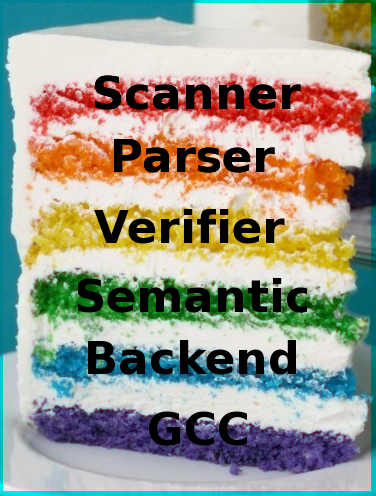
\includegraphics[width=40mm]{figures/layers.png}
\caption{A diagram showing the layers of \sys{}. The raw source code is
fed into the top of the cake and binary executables come out the bottom.
(NOTE: This image was manipulated by \sys{} using a Gaussian blur filter.)}
\label{fig:layers}
\end{center}
\end{wrapfigure}

Our design incorporates six layers: the scanner, the parser, the verifier,
the semantic converter, the backend C generation, and C image manipulation
libraries (see Figure~\ref{fig:layers}). The compiler takes as input
a text file containing a valid \sys{} program and outputs a binary that
implements the program described by the input text.

\begin{figure}
\begin{center}
\begin{tabular}{l l l l l l l}

    SEMI & LPAREN & RPAREN & LTCHAR & GTCHAR & LBRKT & RBRKT \\
    LBRACE & RBRACE & COLON & COMMA & FSLASH & CONVOP & PIPE \\
    ATSYM & UMINUS & UPLUS & ASSIGN & DEFINE & OREQUAL & IMAGET \\
    KERNELT & CALCT & CHANNELT & UINT8T & UINT16T & UINT32T & INT8T \\
    INT16T & INT32T & ANGLET & IMGREAD & IMGWRITE & LITSTR & CSTR \\
    INTEGER & ID & EOF \\

\end{tabular}
\caption{A comprehensive list of tokens produced by the lexical analysis (scanner).}
\label{fig:tokens}
\end{center}
\end{figure}

The scanner generates as its output a one-dimensional list of tokens (see Figure~\ref{fig:tokens}).

The parser reads this token list and uses our context-free grammar to generate
an abstract syntax tree. The parser is not strict about which nodes have
which children, or whether or not it is meaningful to have the current
structure: rather it just blindly assembles the tree. The abstract syntax tree
has the nodes described in Figure~\ref{fig:astnodes}.

\vspace{10mm}
\begin{figure}
\begin{center}
\begin{tabular}{l | l}
{\bf Node} & {\bf Description} \\
\hline \\
stmt & Statement \\
vdecl & Variable Declaration \\
expr & Expression \\
matrix & Calc matrix \\
bareint & Integer \\
kerncalc & Kernel calculation \\
chanref & Image channel reference \\
libfunc & \sys{} library function \\
assign\_op & Assignment operation \\
atom & Atomic type
\end{tabular}
\caption{List of Abstract Syntax Tree Nodes.}
\label{fig:astnodes}
\end{center}
\end{figure}

The verifier accepts as input an abstract syntax tree. It traverses the
tree and checks that nodes are arranged in meaningful ways. While it
traverses, it also builds up an environment that keeps track of all
variables defined, along with their identifier name and type. If the
verifier accepts the AST, it will return as output the cumulative
environment that contains the identifiers and their types.

The semantic converter takes in a verified abstract syntax tree and also the
list of variables generated by the verifier. It then maps each node or
configuration of nodes to a corresponding Semantic AST node that
corresponds more directly with the eventual C code that must be generated.
The output of this layer is a semantically checked abstract syntax tree
(SAST). The semantic converter also supplements the environment information
inherited from the verifier with additional information not related to
verification, such the largest referenced command-line argument.

% TODO: Mapping of AST -> SAST ??

The backend takes as input the SAST and the supplemented environment
information. It then converts this into a meaningful C++ program source
file. This program can be submitted to GCC and compiled.

The final layer of \sys{} is the GCC compiler. The generated C source from
the backend is fed into the GCC compiler, which outputs a binary in
architecture-specific assembly language.

The lead developers for each layer of \sys{} are identified in
Figure~\ref{fig:leads}.


\begin{figure}
\begin{center}
\begin{tabular}{l | l}
{\bf Layer} & {\bf Lead Developer} \\
\hline \\
Unit Tests & Kevin and Yongxu \\
Scanner & Jeremy \\
Parser & Jeremy \\
Verifier & Jeremy / Robert \\
Semantic & Robert \\
Backend & Robert / Jeremy \\
GCC/G++ & Richard Stallman et al. \\
\end{tabular}
\caption{Lead Developer of Each Layer.}
\label{fig:leads}
\end{center}
\end{figure}



    \chapter{Test Plan}
\label{chap:testplan}

Our unit test framework consists of pairs of identically named files in the \texttt{clam/tests/} directory.
Each pair consists of a CLAM program with extension \texttt{.clam} and an executable shell script
with extension \texttt{.test}. The CLAM file contains the code to be tested, while the shell script
specifies how to test that code: whether to compile and run or only compile, whether the test is supposed to fail,
what the expected output should look like, and what command line arguments to pass.
The \texttt{_buildup.sh} sets up the testing environment and defines common procedures such as
\texttt{compile-it} and \texttt{run-it}. Furthermore, \texttt{all.test} runs all tests in the directory,
tallies successes and failures and outputs a summary at the end.

Our testing is divided into four sections: syntax verification (section~\ref{testing:syntax}),
semantic/type verification (section~\ref{testing:semantic}),
CString verification (section~\ref{testing:cstrings}),
and functional output verification (section~\ref{testing:output}) which tests image processing results by comparison.

\section{Syntax Verification}
\label{testing:syntax}

Syntax verification testing is meant to confirm that the parser accepts all valid token strings,
and rejects all invalid ones as defined in our language reference manual.
We achieve this by inspecting \texttt{clam/parser.mly} and writing unit tests for
potentially problematic cases (many of the more straightforward rules were not deemed test-worthy).
All of these tests are only compiled and not executed. The testing process uncovered a number of errors
in matrix parsing and definition of kernel calculation lists.\\

\begin{itemize}

\item \texttt{matrix1.clam} tests that a simple matrix parses correctly, and should compile:
\lstinputlisting[language=CLAM]{../clam/tests/matrix1.clam}
(This originally failed because a scale factor was required, but now it is accepted.)

\item \texttt{matrix2.clam} tests that a matrix with scaling factor parses correctly, and should compile:
\lstinputlisting[language=CLAM]{../clam/tests/matrix2.clam}

\item \texttt{matrix3.clam} tests whether the parser catches ill-formed matrices, and should not compile:
\lstinputlisting[language=CLAM]{../clam/tests/matrix3.clam}
(This originally succeeded due to incorrect matrix parsing rules, but now it fails.)

\item \texttt{matrix4.clam} tests whether the parser catches another type of ill-formed matrix, and should also not compile:
\lstinputlisting[language=CLAM]{../clam/tests/matrix4.clam}
(This originally succeeded due to incorrect matrix parsing rules, but now it fails.)

\item \texttt{keyword-id.clam} tests whether the parser allows keywords to be identifiers, and should not compile:
\lstinputlisting[language=CLAM]{../clam/tests/keyword-id.clam}

\item \texttt{1calc-ker.clam} tests whether the parser allows \texttt{Kernel} definitions with only one \texttt{Calc}, and should compile:
\lstinputlisting[language=CLAM]{../clam/tests/keyword-id.clam}
(This originally failed because the original syntax caused reduce/reduce errors, so we changed both the parser and the test.
There was originally no \texttt{|} after the \texttt{=}.)

\item\texttt{string1.clam} checks that consecutive string literals are
  concatenated together into a single string literal. This should compile:
\lstinputlisting[language=CLAM]{../clam/tests/string1.clam}

\item \texttt{convoperand.clam} tests whether the \texttt{**} enforces a strict order of operands, and should not compile:
\lstinputlisting[language=CLAM]{../clam/tests/convoperand.clam}
(We only allow convolutions of the form \emph{channel-ref} \texttt{**} \emph{identifier}, in order to simplify
to translation into C code.)

\item \texttt{defcalc1.clam}, \texttt{defcalc2.clam}, and \texttt{defcalc3.clam} test various ways of declaring \texttt{Calc}s,
and all three should compile:
\lstinputlisting[language=CLAM]{../clam/tests/defcalc1.clam}
\lstinputlisting[language=CLAM]{../clam/tests/defcalc2.clam}
\lstinputlisting[language=CLAM]{../clam/tests/defcalc3.clam}

\item \texttt{rval-calc.clam}, \texttt{rval-matrix.clam}, \texttt{rval-chanref.clam}, \texttt{rval-conv.clam},
\texttt{rval-cstr.clam}, \texttt{rval-image.clam}, \texttt{rval-imgread.clam}, and \texttt{rval-kernel.clam}
test various "do nothing" statements consisting solely of r-values. Theses should all compile, though their
return values of the last line of each test are discarded so they do nothing:
\lstinputlisting[language=CLAM]{../clam/tests/rval-calc.clam}
\lstinputlisting[language=CLAM]{../clam/tests/rval-matrix.clam}
\lstinputlisting[language=CLAM]{../clam/tests/rval-chanref.clam}
\lstinputlisting[language=CLAM]{../clam/tests/rval-conv.clam}
\lstinputlisting[language=CLAM]{../clam/tests/rval-cstr.clam}
\lstinputlisting[language=CLAM]{../clam/tests/rval-image.clam}
\lstinputlisting[language=CLAM]{../clam/tests/rval-imgread.clam}
\lstinputlisting[language=CLAM]{../clam/tests/rval-kernel.clam}
(The parser accepted all of these, though most originally caused errors in the C translator
that had to be fixed (see "C Compiler Verification" below).)

\item \texttt{equality-trans.clam} checks that assignment expressions can be nested. This should compile:
\lstinputlisting[language=CLAM]{../clam/tests/equality-trans.clam}

\item \texttt{comment1.clam} checks that a program with only a comment (and zero statements) compiles. This should compile:
\lstinputlisting[language=CLAM]{../clam/tests/comment1.clam}

\end{itemize}

\section{Semantic Verification}
\label{testing:semantic}

Semantic verification testing is meant to confirm that the verifier accepts all valid parse trees,
and rejects all invalid ones according to the specifications of our language
(and according to what makes sense).
These tests depend on \texttt{clam/verifier.ml}, as well as \texttt{clam/environ.ml} and \texttt{envtypes.mli}. 
The testing process uncovered a number of errors in matrix verification (separate from syntax)
and the creation of default RGB Channels.\\

\begin{itemize}

\item\texttt{zerocalc1.clam} and \texttt{zerocalc2.clam} check that a matrix scaling-factor can
have a numerator of zero, but not a denominator of zero.
The former should certainly compile, while the latter should not:
\lstinputlisting[language=CLAM]{../clam/tests/zerocalc1.clam}
\lstinputlisting[language=CLAM]{../clam/tests/zerocalc2.clam}
(\texttt{zerocalc2.clam} originally passed verification, but that was fixed.)

\item\texttt{invalid1.clam} checks that undeclared identifiers are caught. This should not compile:
\lstinputlisting[language=CLAM]{../clam/tests/invalid1.clam}

\item\texttt{undefined1.clam} checks that an undefined Channel reference cannot be an r-value. This should not compile:
\lstinputlisting[language=CLAM]{../clam/tests/undefined1.clam}

\item\texttt{imgchannel1.clam} checks that an \texttt{Image} has default channels when read. This should compile:
\lstinputlisting[language=CLAM]{../clam/tests/imgchannel1.clam}

\item\texttt{imgchannel2.clam} checks that an undefined \texttt{Calc} cannot be applied to an \texttt{Image}. This should not compile:
\lstinputlisting[language=CLAM]{../clam/tests/imgchannel2.clam}

\item\texttt{imgchannel3.clam} checks that a \texttt{Calc} defined as a matrix cannot be applied to an \texttt{Image}. This should not compile:
\lstinputlisting[language=CLAM]{../clam/tests/imgchannel3.clam}

\item\texttt{imgchannel4.clam} checks that a \texttt{Calc} defined as a CString \emph{can} be applied to an \texttt{Image}. This should compile:
\lstinputlisting[language=CLAM]{../clam/tests/imgchannel4.clam}

\item\texttt{image-eq-image.clam} checks \texttt{=} assignment for images to images. This should compile:
\lstinputlisting[language=CLAM]{../clam/tests/image-eq-image.clam}

\item\texttt{image-oreq-image.clam} checks \texttt{|=} assignment for images to images. This is not supported and doesn't compile:
\lstinputlisting[language=CLAM]{../clam/tests/image-oreq-image.clam}

\item\texttt{image-defeq.clam} checks \texttt{:=} assignment for images. This is not supported and doesn't compile:
\lstinputlisting[language=CLAM]{../clam/tests/image-defeq.clam}

\item\texttt{imgread-bad.clam} checks that l-value identifiers have to be declared first. This shouldn't compile:
\lstinputlisting[language=CLAM]{../clam/tests/imgread-bad.clam}

\item\texttt{imgread-bad2.clam} checks that \texttt{imgread} must be called with only one argument. This shouldn't compile:
\lstinputlisting[language=CLAM]{../clam/tests/imgread-bad2.clam}

\item\texttt{imgread-bad3.clam} checks that \texttt{imgread} can only be called with a literal string or integer. This shouldn't compile:
\lstinputlisting[language=CLAM]{../clam/tests/imgread-bad3.clam}

\item\texttt{imgread.clam} checks that \texttt{imgread} can actually called with a correct argument. This should compile:
\lstinputlisting[language=CLAM]{../clam/tests/imgread-bad.clam}

\item\texttt{imgwrite-bad1.clam} checks that \texttt{imgwrite} can't be called with incorrect number and type of arguments. This shouldn't compile:
\lstinputlisting[language=CLAM]{../clam/tests/imgwrite-bad1.clam}

\item\texttt{defchannels.clam} checks that the default RGB Channels don't exist for a declared-but-not-read \texttt{Image}. This shouldn't compile:
\lstinputlisting[language=CLAM]{../clam/tests/defchannels.clam}
(Allowing default RGB channels for an unread \texttt{Image} is problematic because CLAM
does not allow explicit manipulation of Channel \emph{size}.)

\item\texttt{imgwrite-norgb.clam} checks that a declared-but-not-read \texttt{Image} without RGB channels
(and more importantly, without a \emph{size}) cannot be written. This shouldn't compile:
\lstinputlisting[language=CLAM]{../clam/tests/imgwrite-norgb.clam}

\item\texttt{sizediff.clam} checks that the default Channels from \texttt{Image}s of different sizes
cannot be assigned to each other, because all Channels of an \texttt{Image} should have the same size. This shouldn't compile:
\lstinputlisting[language=CLAM]{../clam/tests/sizediff.clam}

\item\texttt{at-channel.clam} checks that transient \texttt{Calc}s marked with \texttt{@} in a \texttt{Kernel}
do not result in Channels after a convolution. This shouldn't compile:
\lstinputlisting[language=CLAM]{../clam/tests/at-channel.clam}

\item\texttt{addker.clam} checks a \texttt{Kernel} can be appended to another \texttt{Kernel} using \texttt{|=}. This should compile:
\lstinputlisting[language=CLAM]{../clam/tests/addker.clam}

\item\texttt{DefEq.clam} checks that \texttt{=} cannot be used to define a \texttt{Calc}. This should not compile:
\lstinputlisting[language=CLAM]{../clam/tests/DefEq.clam}

\item\texttt{ckernel.clam} checks that \texttt{Kernel}s must be defined using \texttt{Calc} \emph{identifiers}
and not anonymous \texttt{Calc} expressions. This should not compile:
\lstinputlisting[language=CLAM]{../clam/tests/ckernel.clam}

\item\texttt{cimage.clam} checks that \texttt{Image}s cannot be defined using \texttt{Calc} expressions. This should not compile:
\lstinputlisting[language=CLAM]{../clam/tests/cimage.clam}

\end{itemize}

\section{CString Verification}
\label{testing:cstrings}

CString verification testing checks that invalid CStrings are caught before being passed to GCC, where they
could cause fatal errors. Of course, it is impossible to catch \emph{all} possible errors without
building an understanding of C syntax directly into CLAM, so we are satisfied with catching common
mistakes and rely on the user and GCC error messages for everything else. (For example, a CString of the form \texttt{\#[while(1)]\#},
while certainly disruptive, will compile and it is the user's fault that the program stalls.)
For each possible issue that we \emph{did} choose to catch, we wrote unit tests to confirm that they were caught.
Catching of invalid CStrings is done entirely in \texttt{clam/scanner.mll}. Testing reveals errors
in parentheses matching, which were promptly corrected.\\

\begin{itemize}

\item\texttt{cstring1.clam} checks that C preprocessor cannot be used in a CString. This should not compile:
\lstinputlisting[language=CLAM]{../clam/tests/cstring1.clam}

\item\texttt{cstring2.clam} checks that C comments cannot be used in a CString. This should not compile:
\lstinputlisting[language=CLAM]{../clam/tests/cstring2.clam}

\item\texttt{cstring3.clam} checks that empty CStrings are OK, and just result in an empty statement. This should compile:
\lstinputlisting[language=CLAM]{../clam/tests/cstring3.clam}

\item\texttt{cstring4.clam} checks that library calls in a CString must be closed. This should not compile:
\lstinputlisting[language=CLAM]{../clam/tests/cstring4.clam}
(This originally did compile because the scanner didn't record nesting-level properly. It was fixed.)

\item\texttt{cstring5.clam} checks that parentheses in a CString must be matched. This should not compile:
\lstinputlisting[language=CLAM]{../clam/tests/cstring5.clam}
(This originally did compile because the scanner didn't record nesting-level properly. It was fixed.)

\item\texttt{cstring6.clam} is a sanity check that "normal" CStrings do in fact work. This should obviously compile:
\lstinputlisting[language=CLAM]{../clam/tests/cstring6.clam}

\end{itemize}

\section{C Compiler Verification}
\label{testing:ccompiler}

A few of the above tests, which originally compiled, began failing once the C backend was hooked up.
The most common errors were with C syntax and memory allocation.
While we didn't write tests specifically targeted at the C backend,
the tests we wrote for other parts of the architecture also helped us identify problems in the C translator. 

\section{Image Processing Verification}
\label{testing:output}

These are comprehensive tests, consisting of full-fledged programs that actually
read, manipulate and write images. While the testing framework provides image-comparison functionality,
most verification here is actually done with the naked eye.\\

\begin{itemize}

\item\texttt{imgcopy.clam} copies an image. This should compile, run, and copy an image:
\lstinputlisting[language=CLAM]{../clam/tests/imgcopy.clam}

\item\texttt{sobel.clam} applies the Sobel operation to an image. This should compile, run, and output
a map of the luminosity gradient:
\lstinputlisting[language=CLAM]{../clam/tests/sobel.clam}

\end{itemize}



    \chapter{Lessons Learned}
\label{chap:lessons}

\section{Jeremy Andrus}
Through the course of this project, there are several things that I learned.
First, I learned that writing a compiler is
much more complicated than I had first imagined. While OCaml's syntax and scanner/parser
integration ease development quite a bit, there was still a lot of code to write.
Second, I learned that the implementation of a backend generator, the definition of
a C API that the generator will use, and the syntax tree that the generator takes as
input are all intensely entwined. It was nearly impossible for us to separate the
design of the C/C++ implementation library from the generator backend, and similarly it
was impossible to separate the backend generator design from the abstract syntax tree
that it took as input.

Finally, I learned that self-motivation in a group setting seems to decrease proportionally
to the number of members in the group. Idealistic dreams of independantly motivated
developers all hacking towards a common goal are naive, and more realistic approaches to
group dynamics must be applied. This means that nagging emails and explicit time spent
on planning and organizing will inevitably save late-night hacking cycles near the end
of the project.


\section{Robert Martin}
It's the little things that end up being the big things. When we started
the project, we had a good idea of the functionality we wanted to express
in our language, but we did not precisely work out the gritty details of
the entire translation from \sys{} source code to program execution. We
would have benefited greatly by each writing 1 or 2 example programs before
we had ever written a line of code. We could then have reconvened to talk
through our example programs, discussing at a high level what we would
expect the resultant binary to do at each line and the deductive logic that would
allow it to do so. Such a conversation at an early stage would have exposed
a number of deficiencies and redundancies in the language, and led to a
better finished product.


\section{Kevin Sun}
\begin{itemize}
\item 	Make sure you thoroughly understand the Ocaml examples from class.
\item  	Stay in contact with your team throughout the semester, to make sure 
	everyone is always up to speed.
\item 	Define a clear division of labor early, so work is distributed evenly.
\item 	Do lots of testing, even (especially) for apparently simple cases.
	It's so easy to overlook minor details, and a comprehensive set of tests
	is a great way to ensure you don't break anything.
\item 	At the same time, definitely try to push your language in testing.
	Thinking of ways a coder could break your language forces you to think about
	the details of your implementation.
\end{itemize}




\section{Yongxu Zhang}
Learned in detail how the AST, scanner, parser and verifier are worked together to translate a programming language into an executable. Under some circumstances, it’s not as easy as I thought. For example, one needs to take the precedence and data types check into consideration from very beginning, such as designing a syntax tree. The way in which one part is designed may have significant influence to other parts. When we testing and fixing bugs in syntax, after a lot of syntax errors involving data types were discovered, we rewrote the syntax tree to be strongly typed instead of directly go to modify the parser and verifier, and that saved us a lot of time.

Also I learned how to design unit tests to discover all kinds of dark corners of a language and how to fix them. One cannot follow the routine when designing unit tests. Unusual conditions also need to be considered since they are always useful to detect bugs that out of one’s expectation. By retrieving back to the source code with results of other relative tests, the error is located and fixed.



    \appendix
    \chapter{Complete Code Reference}
\label{chap:coderef}
The \sys{} programming language was implemented in OCaml. It uses the
C/C++ programming languages as backend targets, and invokes the \texttt{g++}
compiler on the \sys{} compilation output to produce a final binary. The
final binary is statically linked against a \sys{} implementation library,
\texttt{clam.a}, which contains the low-level image manipulation functions. Additionally,
\sys{} leveraged several OCaml functions from the \emph{extlib}~\cite{extlib:googlecode}
project, and a stand-alone image reader~\cite{stbimage:read} and writer~\cite{stbimage:write}
library written by Sean Barrett. Code listings of the \sys{} compiler and \sys{} implementation library
as well as the subset of \emph{extlib} used by \sys{} follow:

\clearpage
\section{\sys{} Compiler}
\lstinputlisting[language=Ocaml]{../clam/clam.ml} \clearpage
\lstinputlisting[language=Ocaml]{../clam/ast.mli} \clearpage
\lstinputlisting[language=Ocaml]{../clam/backend.ml} \clearpage
\lstinputlisting[language=Ocaml]{../clam/clamsys.ml} \clearpage
\lstinputlisting[language=Ocaml]{../clam/environ.ml} \clearpage
\lstinputlisting[language=Ocaml]{../clam/envtypes.mli} \clearpage
\lstinputlisting[language=Ocaml]{../clam/parseutil.ml} \clearpage
\lstinputlisting[language=Ocaml]{../clam/parser.mly} \clearpage
\lstinputlisting[language=Ocaml]{../clam/printer.ml} \clearpage
\lstinputlisting[language=Ocaml]{../clam/sast.mli} \clearpage
\lstinputlisting[language=Ocaml]{../clam/scanner.mll} \clearpage
\lstinputlisting[language=Ocaml]{../clam/semantic.ml} \clearpage
\lstinputlisting[language=Ocaml]{../clam/verifier.ml} \clearpage

\subsection{Subset of \emph{extlib} Used by \sys{}}
\sys{} compiled the following source files from the \texttt{extlib}~\cite{extlib:googlecode}
project. Their full source is omitted for brevity -- see the project website.
\begin{itemize}
  \item{\texttt{enum.ml}}
  \item{\texttt{enum.mli}}
  \item{\texttt{extString.ml}}
  \item{\texttt{extString.mli}}
  \item{\texttt{std.ml}}
  \item{\texttt{std.mli}}
\end{itemize}
\comment{
  \lstinputlisting[language=Ocaml]{../clam/extlib/enum.ml} \clearpage
  \lstinputlisting[language=Ocaml]{../clam/extlib/enum.mli} \clearpage
  \lstinputlisting[language=Ocaml]{../clam/extlib/extString.ml} \clearpage
  \lstinputlisting[language=Ocaml]{../clam/extlib/extString.mli} \clearpage
  \lstinputlisting[language=Ocaml]{../clam/extlib/std.ml} \clearpage
  \lstinputlisting[language=Ocaml]{../clam/extlib/std.mli} \clearpage
} % END-COMMENT

\section{\sys{} Implementation Library (\texttt{clam.a})}
\definecolor{cstyleDarkRed}{rgb}{0.65, 0.08, 0.0}
\definecolor{cstyleDarkBlue}{rgb}{0.0, 0.08, 0.65}
\definecolor{cstyleGrey}{rgb}{0.55, 0.55, 0.55}
\lstset{
    keywordstyle={\color{cstyleDarkRed}\bfseries},
    commentstyle={\color{cstyleGrey}\bfseries},
    %directivestyle={\color{cstyleDarkBlue}},
    sensitive=true,
    showstringspaces=false,
    showspaces=false,
    showtabs=false,
    numbers=left,
    frame=single,
    breaklines=true,
    basicstyle=\ttfamily\scriptsize,
}
%\subsection{\sys{} C Source}
\lstinputlisting[language=C]{../clam/libstb/clam.h} \clearpage
\lstinputlisting[language=C]{../clam/libstb/clam.c} \clearpage
%\subsection{\texttt{stb\_image} Source}
%\lstinputlisting[language=C]{../clam/libstb/stb-image-read.c} \clearpage
%\lstinputlisting[language=C]{../clam/libstb/stb-image-write.c} \clearpage

\section{Unit Test Framework}
Our unit testing framework was built on two custom shell scripts that provided
a framework to compile a test program, determine success/failure of compilation,
compare image outputs and report overall success or failure of the test.
The framework simply runs all shell scripts in the \emph{test} directory and
reports the success/failure of each one (with a summary of failures at the end).
The \texttt{_buildup.sh}, \texttt{_breakdown.sh}, and \texttt{all.test} scripts are
reported here, followed by all of the tests and a sample run of the
\texttt{all.test} script.
\vskip -4mm

\vskip -4mm
\subsection*{_buildup.sh}
\vskip -2mm
\lstinputlisting[language=bash]{../clam/tests/build-up-script-link.sh} \clearpage
\subsection*{_breakdown.sh}
\lstinputlisting[language=bash]{../clam/tests/breakdown-script-link.sh}
\subsection*{all.test}
\lstinputlisting[language=bash]{../clam/tests/all.test} \clearpage
% all the tests 
\subsection*{The tests (shell script followed by \sys{} source)}
\subsection*{Unit Test: 1calc-ker}
\lstinputlisting[language=bash]{../clam/tests/1calc-ker.test}
\lstinputlisting[language=CLAM]{../clam/tests/1calc-ker.clam} \clearpage
\subsection*{Unit Test: DefEq}
\lstinputlisting[language=bash]{../clam/tests/DefEq.test}
\lstinputlisting[language=CLAM]{../clam/tests/DefEq.clam} \clearpage
\subsection*{Unit Test: addker}
\lstinputlisting[language=bash]{../clam/tests/addker.test}
\lstinputlisting[language=CLAM]{../clam/tests/addker.clam} \clearpage
\subsection*{Unit Test: at-channel}
\lstinputlisting[language=bash]{../clam/tests/at-channel.test}
\lstinputlisting[language=CLAM]{../clam/tests/at-channel.clam} \clearpage
\subsection*{Unit Test: cimage}
\lstinputlisting[language=bash]{../clam/tests/cimage.test}
\lstinputlisting[language=CLAM]{../clam/tests/cimage.clam} \clearpage
\subsection*{Unit Test: ckernel}
\lstinputlisting[language=bash]{../clam/tests/ckernel.test}
\lstinputlisting[language=CLAM]{../clam/tests/ckernel.clam} \clearpage
\subsection*{Unit Test: comment1}
\lstinputlisting[language=bash]{../clam/tests/comment1.test}
\lstinputlisting[language=CLAM]{../clam/tests/comment1.clam} \clearpage
\subsection*{Unit Test: convoperand}
\lstinputlisting[language=bash]{../clam/tests/convoperand.test}
\lstinputlisting[language=CLAM]{../clam/tests/convoperand.clam} \clearpage
\subsection*{Unit Test: cstring1}
\lstinputlisting[language=bash]{../clam/tests/cstring1.test}
\lstinputlisting[language=CLAM]{../clam/tests/cstring1.clam} \clearpage
\subsection*{Unit Test: cstring2}
\lstinputlisting[language=bash]{../clam/tests/cstring2.test}
\lstinputlisting[language=CLAM]{../clam/tests/cstring2.clam} \clearpage
\subsection*{Unit Test: cstring3}
\lstinputlisting[language=bash]{../clam/tests/cstring3.test}
\lstinputlisting[language=CLAM]{../clam/tests/cstring3.clam} \clearpage
\subsection*{Unit Test: cstring4}
\lstinputlisting[language=bash]{../clam/tests/cstring4.test}
\lstinputlisting[language=CLAM]{../clam/tests/cstring4.clam} \clearpage
\subsection*{Unit Test: cstring5}
\lstinputlisting[language=bash]{../clam/tests/cstring5.test}
\lstinputlisting[language=CLAM]{../clam/tests/cstring5.clam} \clearpage
\subsection*{Unit Test: cstring6}
\lstinputlisting[language=bash]{../clam/tests/cstring6.test}
\lstinputlisting[language=CLAM]{../clam/tests/cstring6.clam} \clearpage
\subsection*{Unit Test: defcalc1}
\lstinputlisting[language=bash]{../clam/tests/defcalc1.test}
\lstinputlisting[language=CLAM]{../clam/tests/defcalc1.clam} \clearpage
\subsection*{Unit Test: defcalc2}
\lstinputlisting[language=bash]{../clam/tests/defcalc2.test}
\lstinputlisting[language=CLAM]{../clam/tests/defcalc2.clam} \clearpage
\subsection*{Unit Test: defcalc3}
\lstinputlisting[language=bash]{../clam/tests/defcalc3.test}
\lstinputlisting[language=CLAM]{../clam/tests/defcalc3.clam} \clearpage
\subsection*{Unit Test: defchannels}
\lstinputlisting[language=bash]{../clam/tests/defchannels.test}
\lstinputlisting[language=CLAM]{../clam/tests/defchannels.clam} \clearpage
\subsection*{Unit Test: equality-trans}
\lstinputlisting[language=bash]{../clam/tests/equality-trans.test}
\lstinputlisting[language=CLAM]{../clam/tests/equality-trans.clam} \clearpage
\subsection*{Unit Test: id-overlap}
\lstinputlisting[language=bash]{../clam/tests/id-overlap.test}
\lstinputlisting[language=CLAM]{../clam/tests/id-overlap.clam} \clearpage
\subsection*{Unit Test: image-defeq}
\lstinputlisting[language=bash]{../clam/tests/image-defeq.test}
\lstinputlisting[language=CLAM]{../clam/tests/image-defeq.clam} \clearpage
\subsection*{Unit Test: image-eq-image}
\lstinputlisting[language=bash]{../clam/tests/image-eq-image.test}
\lstinputlisting[language=CLAM]{../clam/tests/image-eq-image.clam} \clearpage
\subsection*{Unit Test: image-oreq-image}
\lstinputlisting[language=bash]{../clam/tests/image-oreq-image.test}
\lstinputlisting[language=CLAM]{../clam/tests/image-oreq-image.clam} \clearpage
\subsection*{Unit Test: imgchannel1}
\lstinputlisting[language=bash]{../clam/tests/imgchannel1.test}
\lstinputlisting[language=CLAM]{../clam/tests/imgchannel1.clam} \clearpage
\subsection*{Unit Test: imgchannel2}
\lstinputlisting[language=bash]{../clam/tests/imgchannel2.test}
\lstinputlisting[language=CLAM]{../clam/tests/imgchannel2.clam} \clearpage
\subsection*{Unit Test: imgchannel3}
\lstinputlisting[language=bash]{../clam/tests/imgchannel3.test}
\lstinputlisting[language=CLAM]{../clam/tests/imgchannel3.clam} \clearpage
\subsection*{Unit Test: imgchannel4}
\lstinputlisting[language=bash]{../clam/tests/imgchannel4.test}
\lstinputlisting[language=CLAM]{../clam/tests/imgchannel4.clam} \clearpage
\subsection*{Unit Test: imgcopy}
\lstinputlisting[language=bash]{../clam/tests/imgcopy.test}
\lstinputlisting[language=CLAM]{../clam/tests/imgcopy.clam} \clearpage
\subsection*{Unit Test: imgread}
\lstinputlisting[language=bash]{../clam/tests/imgread.test}
\lstinputlisting[language=CLAM]{../clam/tests/imgread.clam} \clearpage
\subsection*{Unit Test: imgread-bad}
\lstinputlisting[language=bash]{../clam/tests/imgread-bad.test}
\lstinputlisting[language=CLAM]{../clam/tests/imgread-bad.clam} \clearpage
\subsection*{Unit Test: imgread-bad2}
\lstinputlisting[language=bash]{../clam/tests/imgread-bad2.test}
\lstinputlisting[language=CLAM]{../clam/tests/imgread-bad2.clam} \clearpage
\subsection*{Unit Test: imgread-bad3}
\lstinputlisting[language=bash]{../clam/tests/imgread-bad3.test}
\lstinputlisting[language=CLAM]{../clam/tests/imgread-bad3.clam} \clearpage
\subsection*{Unit Test: imgwrite-bad1}
\lstinputlisting[language=bash]{../clam/tests/imgwrite-bad1.test}
\lstinputlisting[language=CLAM]{../clam/tests/imgwrite-bad1.clam} \clearpage
\subsection*{Unit Test: imgwrite-norgb}
\lstinputlisting[language=bash]{../clam/tests/imgwrite-norgb.test}
\lstinputlisting[language=CLAM]{../clam/tests/imgwrite-norgb.clam} \clearpage
\subsection*{Unit Test: invalid1}
\lstinputlisting[language=bash]{../clam/tests/invalid1.test}
\lstinputlisting[language=CLAM]{../clam/tests/invalid1.clam} \clearpage
\subsection*{Unit Test: keyword-id}
\lstinputlisting[language=bash]{../clam/tests/keyword-id.test}
\lstinputlisting[language=CLAM]{../clam/tests/keyword-id.clam} \clearpage
\subsection*{Unit Test: matrix1}
\lstinputlisting[language=bash]{../clam/tests/matrix1.test}
\lstinputlisting[language=CLAM]{../clam/tests/matrix1.clam} \clearpage
\subsection*{Unit Test: matrix2}
\lstinputlisting[language=bash]{../clam/tests/matrix2.test}
\lstinputlisting[language=CLAM]{../clam/tests/matrix2.clam} \clearpage
\subsection*{Unit Test: matrix3}
\lstinputlisting[language=bash]{../clam/tests/matrix3.test}
\lstinputlisting[language=CLAM]{../clam/tests/matrix3.clam} \clearpage
\subsection*{Unit Test: matrix4}
\lstinputlisting[language=bash]{../clam/tests/matrix4.test}
\lstinputlisting[language=CLAM]{../clam/tests/matrix4.clam} \clearpage
\subsection*{Unit Test: rval-calc}
\lstinputlisting[language=bash]{../clam/tests/rval-calc.test}
\lstinputlisting[language=CLAM]{../clam/tests/rval-calc.clam} \clearpage
\subsection*{Unit Test: rval-chanref}
\lstinputlisting[language=bash]{../clam/tests/rval-chanref.test}
\lstinputlisting[language=CLAM]{../clam/tests/rval-chanref.clam} \clearpage
\subsection*{Unit Test: rval-conv}
\lstinputlisting[language=bash]{../clam/tests/rval-conv.test}
\lstinputlisting[language=CLAM]{../clam/tests/rval-conv.clam} \clearpage
\subsection*{Unit Test: rval-cstr}
\lstinputlisting[language=bash]{../clam/tests/rval-cstr.test}
\lstinputlisting[language=CLAM]{../clam/tests/rval-cstr.clam} \clearpage
\subsection*{Unit Test: rval-image}
\lstinputlisting[language=bash]{../clam/tests/rval-image.test}
\lstinputlisting[language=CLAM]{../clam/tests/rval-image.clam} \clearpage
\subsection*{Unit Test: rval-imgread}
\lstinputlisting[language=bash]{../clam/tests/rval-imgread.test}
\lstinputlisting[language=CLAM]{../clam/tests/rval-imgread.clam} \clearpage
\subsection*{Unit Test: rval-kernel}
\lstinputlisting[language=bash]{../clam/tests/rval-kernel.test}
\lstinputlisting[language=CLAM]{../clam/tests/rval-kernel.clam} \clearpage
\subsection*{Unit Test: rval-matrix}
\lstinputlisting[language=bash]{../clam/tests/rval-matrix.test}
\lstinputlisting[language=CLAM]{../clam/tests/rval-matrix.clam} \clearpage
\subsection*{Unit Test: sizediff}
\lstinputlisting[language=bash]{../clam/tests/sizediff.test}
\lstinputlisting[language=CLAM]{../clam/tests/sizediff.clam} \clearpage
\subsection*{Unit Test: sobel}
\lstinputlisting[language=bash]{../clam/tests/sobel.test}
\lstinputlisting[language=CLAM]{../clam/tests/sobel.clam} \clearpage
\subsection*{Unit Test: string1}
\lstinputlisting[language=bash]{../clam/tests/string1.test}
\lstinputlisting[language=CLAM]{../clam/tests/string1.clam} \clearpage
\subsection*{Unit Test: undefined1}
\lstinputlisting[language=bash]{../clam/tests/undefined1.test}
\lstinputlisting[language=CLAM]{../clam/tests/undefined1.clam} \clearpage
\subsection*{Unit Test: zerocalc1}
\lstinputlisting[language=bash]{../clam/tests/zerocalc1.test}
\lstinputlisting[language=CLAM]{../clam/tests/zerocalc1.clam} \clearpage
\subsection*{Unit Test: zerocalc2}
\lstinputlisting[language=bash]{../clam/tests/zerocalc2.test}
\lstinputlisting[language=CLAM]{../clam/tests/zerocalc2.clam} \clearpage

\chapter{Project Version Control History}
\label{chap:vcshistory}
The \sys{} project used \texttt{git}~\cite{git:website} as its version control system.
Here we provide the output of the \texttt{git-shortlog} program with \emph{Merge}
commits filtered out, followed by a more complete revision control history.

\section{Project Repository \texttt{git} 'shortlog'}
\lstset{numbers=none,frame=none}
\begin{lstlisting}
 ():

\end{lstlisting}

\clearpage
\section{Full \texttt{git} Log}
The following log was generated using the command:
\begin{lstlisting}
git log --color --stat --no-merges --pretty=format:"%h: %Cblue%aN <%aE>%Creset%nDate: %aD%nSubject: %s%nContent: %b"
\end{lstlisting}
\lstset{escapeinside=`'}
\begin{lstlisting}
\end{lstlisting}


    \clearpage
  \fi
  {
    \balance
    \bibliographystyle{abbrv}
    \bibliography{clam}
  }
\fi

\end{document}
